\section{Introduction}
\label{sec:introduction}
%p1 Context
%p2 Problem
%p3 Solution
%p4 Why new
%p5 structure of paper

%     P1: Context
%    
%     P2: Problem
%    
%     P3: Solution
%    
%     P4: Why new
%    
%     P5: Structure of paper

%	+ 1 pages: stable the main goals of your work
%   	+ Context+to get the idea -> 1 paragraph (no citation)
%   	+ Problem + Citations -> <20 lines
%   	+ Approach + Solution -> <20 lines
%   	+ [Why you are novel]
%   	+ Structure of paper, by section -> <20 lines
     
%\textbf{Context + to get the idea -> 1 paragraph (no citation)}

%Neuroimaging techniques allow researchers and clinicians to gain insights of unprecedented quality on the cerebral anatomy. Three main focuses of neuroimaging include \textit{brain decoding}, \textit{brain mapping} and \textit{brain connectivity}. Both brain mapping and brain decoding concern about the prediction or detection of a cognitive stimulus given a recording brain activity and reverse. Contrast with them, 
In neuroimaging, brain connectivity refers to building a model of the connections between different brain areas. \textit{Functional connectivity} focuses on the temporal correlation between the brain activity of anatomically remote areas. \textit{Effective connectivity} investigates causal links between different brain structures. \textit{Anatomical connectivity} refers to the structural links between different areas that develop in the white matter of the brain. Anatomical connectivity is the main focus of this work. 
%Before going on more detail, it is necessary to define some terms that will be used in this paper:
%\begin{itemize}
%	\item \textit{\textbf{Streamline}} is an approximation of about $\sim10K$ neuronal axons sharing the same structural connectivity path. In some cases, \textit{streamline} is also called \textit{\textbf{track}} or \textit{\textbf{fiber}}.
	%, both of which more refers to the mathematical representation.
%	 \item The whole set of \textit{streamlines} of a brain is called \textit{\textbf{tractography}}. And given that the resolution of modern MRI scanners is in the order of $1mm^3$, a full brain tractography consists of $\approx3\times10^5$ streamlines. (see Figure~\ref{fig:tractography})
%	  \item \textit{\textbf{Bundle}} is a set of streamlines with similar spatial and shape characteristics e.g. they are close to each other according to a streamline distance.
%	  \item \textit{\textbf{Tract}} is the real anatomical group of neuronal axons.
%\end{itemize}   
%More recently, several groups have proposed tractography methods and have reported success in following fiber tracts~\cite{zhang2008identifying}.
%\textbf{Problem + Citations -> <20 lines}
Currently, diffusion magnetic resonance imaging (dMRI) techniques are commonly used to find the anatomical connectivity in brain~\cite{basser1994diffusion,tuch2002high}. dMRI is a set of methods for measuring the displacement distribution of water molecules in vivo. From the displacement distribution, we can infer the fiber orientation or orientations in each imaging volume element, called \emph{voxel}, and that allows to reconstruct white matter fiber tracts as a set of \emph{streamlines}. A streamline is an approximation of about $\sim10^3$ neuronal axons sharing the same structural connectivity path. A set of streamlines with similar spatial and shape characteristics is called \emph{bundle}. The whole set of streamlines of a brain is called \emph{tractography}. More recently, several groups have proposed tractography methods and reported success in following fiber tracts (for example deterministic tractography algorithms~\cite{mori2002fiber},\cite{garyfallidis2012towards}). 
One problem raises is how to group streamlines belonging to a common anatomical area into one segmentation. This task is known as \emph{tract segmentation}.
%However, the segmentation process is really slow and requires experience from neuroanatomists. Moreover, the variability of the brain anatomy among different subjects makes the segmentation become a difficult task~\cite{bozzali2002white}.
%\begin{figure*}
%  \centering
%  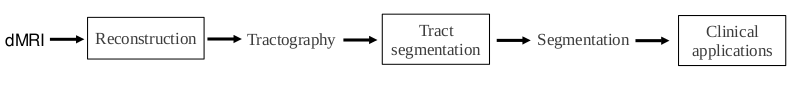
\includegraphics[width=16.2cm, height=1.27cm ]{figures/ov_research2.png}
%  \caption{Tract segmentation takes as input a huge tractography, the result of reconstruction step done on original dMRI data. It produces as output a tract segmentation, which is then used in clinical applications}
%  \label{fig:ov_research}
%\end{figure*}

%\textbf{Approach + Solution -> <20 lines}
Traditionally the segmentation task is done by neuroanatomists, and it consumes a lot of time and effort due to the large number of streamlines (about $3 \times 10^5$ in a normal brain). Moreover, the variability of the brain anatomy among different subjects makes the segmentation become a difficult task~\cite{bozzali2002white}. Recently, the literature about machine learning techniques to solve this problem is increasing. Up to now, there are two approaches for tractography segmentation: supervised~\cite{caruna2006emperical} and unsupervised~\cite{ghahramani2004unsupervised} learning. The unsupervised techniques often rely on expert-crafted streamline-streamline distance functions~\cite{dubuisson1994modified, zhang2008identifying} encoding informative relationships for the segmentation task, then followed by a clustering algorithm (agglomerative, k-means, Gaussian mixture model, etc. see~\cite{wang2011tractography} for a recent brief review). Supervised tract segmentation~\cite{caruna2006emperical,olivetti2011supervised} instead aims at learning how to segment the tractography from expert-made examples provided as input. Although both supervised and unsupervised techniques get some encouraging results, but they are below the expectation of medical practitioners. Unsupervised techniques usually work on the whole tractography while medical practitioner often focus on a specific tract. In the case of supervised learning, the lack of ground truth data makes the results be not good and need the refinement from experts. 
%Moreover, both of them are off-line methods which require the refinement from experts. 

This research is motivated by the need for interaction of medical pratitioners when they do the tract segmentation task. It is impossible for them to have a look at the whole tractography of a brain due to the huge number of streamlines ($\approx 3 \times 10^5$). And it is often an important requirement to view the tractography at different partial views. Medical practitioners usually changes between these levels for better visualization. This demand raises a question of how we can present the whole tractography at different level of zooming in $3D$ space? 

Currently, both supervised and unsupervised learning are unsatisfactory. In this work, we want improve the support of machine learning for the segmentation task. In another way, we want to help medical practitioner to do the segmentation task more easily, and more accurately based on machine learning. More precisely, following are things we want to investigate in this project.
%In this project, following are what we want to investigate:
\\\textbf{Brain tractography segmentation:} In %A novel contribution of 
this work, we combine both \textit{unsupervised} and \textit{supervised} learning to do the task of segmentation. The reason is that each technique is suitable for different steps in the whole process. The framework of our process is showed in the figure \ref{fig:ov_tool}. First, supervised learning is used in the tract identification stage to create the tentative segmentation. Then, this candidate is interactively refined by experts based on fast clustering technique.
\textbf{\textit{Multimodal brain image visualization:}} In order to help medical practitioners to do the segmentation task more easily, and faster, we provide an interactive visualization tool for a large volume brain imaging data in $3D$ space, which is the implementation of our proposed framework for tract segmentation. In this scientific interactive tool, we present a simple way to interact and to segment streamlines, which goes, as far as we know, beyond any other available medical imaging software.
%This method takes as input a huge brain tractography plus the repository of manual segmentation examples, and produces as output a segmentation after refining by experts. 
%To help user can use it friendly, easily, beside the main functions (select/deselect bundle, explore bundle, move/hide slice,etc...) some other common tasks should be integrated such as undo, save current work, load the previous work, etc.
% to help them interact with tracts easier and faster.
%\par{}
%%\textbf{How we can do this?} 
%\textbf{\textit{Supervised tract segmentation:%Multimodal brain image pattern classification methods }} to classify brain tractography into a specific group using supervised learning technique. The idea of the supervised learning is to exploit examples of manually segmented tracts to learn how to extract them automatically from new subjects. This motivation raises from working with doctors and neuroscientists who have already collected many segmented tractogarphy data but it is very difficult for them to use the knowledge in this data for segmentation the new brain. With supervised learning technique, firstly it is necessary to collect enough the manually segmented tractography data. After that, a system will automatic extract some common features from this dataset. These features will be put into a classifier kernel as the standard to classify the tracts belong to which segmentation. At the first idea, some useful features could be the size of bundle, the number of tracts, the length of tracts. This method focuses on the potential benefit of adapting the model learnt from one subject to an other subject. 
%\par{}
%\textbf{\textit{Fast clustering:}} in contrast with the supervised learning, the unsupervised method requires no prior knowledge from neuroscientists. Such techniques often rely on expert-crafted streamline-streamline distance functions encoding informative relationships for the segmentation task, then followed by a clustering algorithm (agglomerative, k-means, Gaussian mixture model, etc. see~\cite{wang2011tractography} for a recent brief review). Due to the fact that result of the classification based on supervised learning usually does not satisfy the requirement of the doctors/neural scientists, it is necessary to let them refine the segmentation again with the help of fast clustering technique. 
%After projecting the tractography into a vector space, one algorithm for clustering the projected tractography can be used. 
%The first idea is to use hierarchical clustering techniques. The motivation behind this is that this algorithm does not base on a specific number of cluster centers. It creates the whole clusters in a hierarchical tree, and when users change the number of cluster, the result of different clusters or segmentations will be appeared. This clustering technique do help doctors/neural scientists to do the segmentation refinement task easier, faster and instantly.
%seperate  swe want to cross-validate the result to know which method has the senior advantage for segmentation tractography task. With the unsupervised method, it requires no prior knowledge from neuroscientists. Such techniques often rely on expert-crafted streamline-streamline distance functions encoding informative relationships for the segmentation task, then followed by a clustering algorithm (agglomerative, k-means, Gaussian mixture model, etc. see~\cite{wang2011tractography} for a recent brief review). 
% In the other side, the idea of the supervised learning is to exploit examples of manually segmented tracts to learn how to extract them automatically from new subjects. This motivation raises from working with doctors and neuroscientists who have already collected many segmented tractogarphy data but it is very difficult for them to use the knowledge in this data for segmentation the new brain. The challenge is to design an effective computational supervised learning approach for tract segmentation in contrast to unsupervised approach.\\
%\par{}
%\textbf{\textit{Dissimilarity approximation:}} both supervised and unsupervised segmentation method base on machine learning technique which requires the input to be from a vectorial space. This requirement contrasts with the intrinsic nature of the tractography because its basic elements, called streamlines or tracks, have different lengths and different number of points and for this reason they cannot be directly represented in a common vectorial space. This lack of the vectorial representation avoids the use of some of those algorithms and of computationally efficient implementations. The dissimilarity space representation could be the way to provide such a vectorial representation and for this reason it is crucial to assess the currently machine learning techniques. Actually, the dissimilarity representation is an Euclidean embedding technique defined by selecting a set of objects (e.g. a set of streamlines) called \emph{prototypes}, and then by mapping any new object (e.g. any new streamline) to the vector of distances from the prototypes. This representation~\cite{pekalska2002generalized,balcan2008theory,chen2009similarity} is usually presented in the context of classification and clustering problems. More detail about this can be found in the section \ref{subsec:dissimilarity}.
\textbf{\textit{Clinical applications:}}
%computer aided diagnosis and follow-up of brain diseases via multimodal images, early diagnosis of brain diseases via multimodal images, and differential diagnosis of brain diseases via multimodal images. 
%\textbf{How we can do this?} \textbf{- clinical diagnosing applications}
The result of tract segmentation is applied to computer aided early diagnosis brain diseases. At a preliminary application, we want to find what differs between the healthy brain and the diseased brain of patients with the ALS disease (Amyotrophic Lateral Sclerosis)\footnote{\url{http://www.alsa.org/about-als/what-is-als.html}}. 
%For this purpose, the diagnosing can be evaluated based on a set of quantitative and qualitative criteria. The qualitative evaluation of the tract reconstruction will be only performed by expert neurosurgeons and radiologists. Therefore, in this work, the main focus is the quantitative criteria which provide useful information for diagnosing brain diseases. Some useful quantitative signal can be used such as fiber profile on diffusion parameters (FA - fractional anisotropy, MD - mean diffusion, eigenvalues ($<\lambda_1,\lambda_2,\lambda_3>$)), correlation and absolute profile distance measures, fiber geometry of volumetric overlap, and the Hausdorff distances between bundles. These parameters are hints for diagnosing some brain diseases, and we here focus on the ALS (Amytrophy Lateral Smytrophic) disease.

%In this work, we want to build an interaction visualization tool that can help instantly medical practitioners to do the segmentation online. This interaction tool uses technique of both supervised (at the first step - hypo generation) and unsupervised learning (at the second step - tract refinement). The frame work of our project is described in the figure \ref{fig:ov_research}, while detail of two main steps of our interactive visualization tool can be found in the figure \ref{fig:ov_tool}
%Instead of using supervised~\cite{caruna2006emperical} and unsupervised~\cite{ghahramani2004unsupervised} machine learning techniques to get the segmentation, we propose the \emph{fast clustering} techniques. Because both supervised and unsupervised learning are off-line method, while in this work, we want to build a tool that can help instantly doctors/neuro scientists to do the segmentation online. 
%We use both supervised~\cite{caruna2006emperical} and unsupervised~\cite{ghahramani2004unsupervised} machine learning techniques to get the segmentation for the whole brain and to compare the results. The unsupervised techniques often rely on expert-crafted streamline-streamline distance functions~\cite{dubuisson1994modified, zhang2008identifying} encoding informative relationships for the segmentation task, then followed by a clustering algorithm (agglomerative, k-means, Gaussian mixture model, etc. see~\cite{wang2011tractography} for a recent brief review). Supervised tract segmentation instead aims at learning how to segment the tractography from expert-made examples provided as input. Up to present, there is a little attention in the literature about supervised tract segmentation.
%\textbf{Summary of the next sections}
%\section{State of the art}
\label{sec:state_of_the_art}
%\subsection{\textbf{About dMRI and deterministic tractography}}
%Scientists in neuroscience seek to gain knowledge of the physical processes that underlie human sensation, attention awareness and cognition. These results are immediately applicable to surgical intervention, to the design of medical interventions and to the treatment of psychological and psychiatric disorders. However, the understanding of the brain, up to present, is currently still an uncover problem. 

%In recent years, \textbf{dMRI-Diffusion Magnetic Resonance Imaging} has gained tremendous popularity in neuro community and became one of the first methods that made it possible to visualize and quantify the organization of white matter in the human brain in vivo.
%\textbf{dMRI-Diffusion Magnetic Resonance Imaging} is evolving into a potent tool in the examination of the central nervous system. 
%Actually, it is a technique that measures local diffusivity of water within the tissue and provides information about the orientation of white matter fiber tracts.
%produces in vivo images of biological tissues by exploiting the constrained diffusion properties of water molecules. In neuroscience,
%dMRI is usually used to extract neuronal fibers from brain dMRI and it offers a good look into brain micro-structure at a scale that is not easily accessible with other modalities, in some cases improving the detection and characterization of white matter abnormalities. 
%Because of that, dMRI can help understand brain connectivity deeply, that has lead to numerous beneficial in both diagnosis and clinical applications. More 
Recently, several groups have proposed tractography methods for reconstruction the whole brain tractography from dMRI data~\cite{zhang2008identifying}. The most popular is the \textbf{deterministic tractography} algorithms~\cite{mori2002fiber}
%, by which we can reconstruct the whole brain tractography from dMRI data. and have reported success in following fiber tracts
An example of the partial tractography extracting from dMRI by using deterministic algorithm is shown in figure \ref{fig:tractography}.
%From dMRI data, the local fiber orientation distribution can be inferred and white matter fiber trajectories as a set of \emph{streamlines} can be reconstructed using the \textbf{deterministic tractography} algorithms~\cite{mori2002fiber}. 
%A \textbf{streamline} is a vectorial representation of thousands of neighboring neuronal axons sharing the same structural connectivity path. The whole set of streamlines of a brain is called \textbf{tractography} (see Figure~\ref{fig:tractography}). The resolution of modern MRI scanners is in the order of $1mm^3$, a full brain tractography consists of $\approx 3 \times 10^5$ streamlines.
\begin{figure}
  \centering
  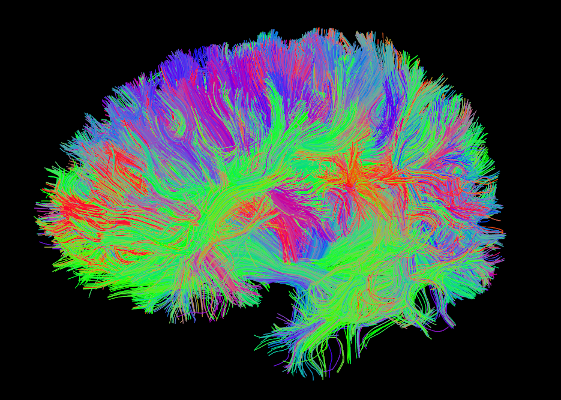
\includegraphics[width=3.18cm, height=2.2cm ]{figures/tractography.png}
  \caption{A tractography of $\approx 3\times 10^5$ streamlines within a brain. 
%(whole set of polylines) made of $\approx 3\times 10^5$ streamlines (polylines) describes the pathways of neural axons within the brain.
	Each single streamlines represents thousands of neighboring neuronal axons expressing structural connectivity.
	Only $3\%$ of the streamlines are shown to improve readability. 
	%Colors represents the main direction of each streamline.
	}
  \label{fig:tractography}
\end{figure}
%-------------------------------------------------------------------------------------------------------
%\subsection{\textbf{About Tractography segmentation}}
However, the resulting tractography datasets are highly complex and include thousands of fibers (about $\approx 3 \times 10^5$), which requires techniques or method to create the exact anatomic brain before doing further studying. The \textbf{segmentation} aims at doing this task, groups some fiber tracts belonging to a common anatomical area into one segmentation. Due to the fact that the complex tractography datasets present a large amount of short association bundles which have been rarely studied until now, it is extremely difficult to cluster some fibers having the same anatomical structure into a group. The segmentation of fiber bundles is therefore a complex and not completely solved problem. 
%Furthermore, clinical studies often use the segmentation of white matter bundles in order to perform comparisons between populations. This is also an press on the accuracy of the segmentation task. 
%The next goal is how we can group some fiber tracks which has the same function into \emph{the specific anatomically structures}. This \textbf{segmentation of the neural streamlines} is a task of interest in neurological studies, for example for the study of Alzheimer disease~\cite{bozzali2002white}. Unlike a simplistic bundle model, where known white matter tracts are represented by a relatively small number of fibers with the same shape, current tractography datasets reconstruct tracts represented by thousands of fibers, composed of various fiber fascicles of different shapes and lengths. 
%Several examples of decomposition of major fiber tracts were already proposed~\cite{lawes2008atlas}. 
%Also, these complex tractography datasets present a large amount of short association bundles, that have been rarely studied until now. Due to the large number of streamlines in a brain (about $\approx 3 \times 10^5$), it is extremely difficult to cluster some streamlines having the same anatomically structure into a group. The segmentation of fiber bundles is therefore a complex and not completely solved problem. 
Recently, the literature about machine learning techniques to solve this problem is increasing. 
%Recently, there is a rise of applying pattern recognition techniques to solve this problem. %Our goal is to applying machine learning techniques to segment the fiber bundles of the human brain. 
In the following part, the brief survey about currently trends in segmentation tractography are presented.

\textbf{\textit{Atlas approach}}
%from Elestherios 78
%To avoid the difficulty of choosing number of clusters, using atlas as prior knowledge is another approach. 
Atlas are the models of white mater structure in brain. 
%The number of clusters is already defined in this atlas, and this leads to no cluster center selection. 
Firstly, atlas are created from experience of experts without being driven from data. After that, atlas are used as model of clusters for tractography segmentation. All streamlines would be grouped into the closest cluster in atlas. O'Donnell and Westin~\cite{odonnell2007automatic} generated a tractographic atlas using spectral embedding and expert anatomical labeling. They then automatically segmented the new tractography using again spectral clustering and embedding the tracks as points in the embedded space, to the closest existing atlas clusters. The true affinity matrix was too big to compute therefore they used the Nystrom approximation: working on a subset and avoid generating the complete distance matrix. However, the important information from the full data set may be lost after sub-sampling. The other main issue of this approach is that up to present, there is no believable algorithm for co-registration two anatomical brains due to the difference of size, position, and direction of these brains.

\textbf{\textit{ROI - region of interest}}
%from Elestherios 78
One of the first idea for segmentation is to use the region of interest (ROI)~\cite{wakana2007reproducibility}. This approach tried to reconstruct tracts passing through ROI by exploiting existing anatomical knowledge of tract trajectories. First, some target tracts must be defined. It also requires to specified manually some regions where tracts start, end or pass through. Then streamlines would be filtered based on the constraint of passing through ROIs. ROI approach needs a priori knowledge about the trajectory and is used only for well-characterized white matter tracts.  
%First, tracking was performed from all pixels inside the brain (brute-force approach)~\cite{hua2008tract}. And results penetrating the manually defined ROIs were assigned to the specific tracts associated with the ROIs. 
In order to refine the segmentation, multi-ROIs were used to include or exclude tracks.
%generated by FACT and Hua et al. [67] used regions of interest together with probabilistic tractography. Zvitia et al. [159], [160] used adaptive mean shift so that they do not need to provide the number of clusters, they also used this approach for registration of datasets from the same subject.

\textbf{\textit{Unsupervised learning }}%without dissimilarity approach} %(in wang2011tractography)
From the point of view of algorithmic approaches, the segmentation task has traditionally been addressed with unsupervised techniques over only diffusion data~\cite{zhang2008identifying}. This typical framework first defines a pairwise distance between fibers and inputs the similarity matrix to standard clustering algorithms. Various distance functions between fibers have been proposed: the Euclidean distances between fiber shape descriptors~\cite{brun2004clustering}; the similarity between two fibers based on the number of points sharing the same voxel~\cite{jonasson2005fiber}; distance from the B-spline representation~\cite{maddah2005automated} ; closest point distance, mean of closest distances and Hausdorff distance~\cite{gerig2004analysis}. Then, following is a clustering algorithm (agglomerative, k-means, Gaussian mixture model, etc. see~\cite{wang2011tractography} for a recent brief review of applying these algorithm for tractography).
%Such techniques often rely on expert-crafted streamline-streamline distance functions encoding informative relationships for the segmentation task.
\\The disadvantage of these clustering algorithms is that they require manually specifying the number of clusters or a threshold for decide when to stop merging or splitting clusters. The different numbers of chosen clusters vary significantly the performance of clustering~\cite{moberts2005evaluation}. 
%In the case that the datasets are complicated and noisy, both of them are difficult to specify. 
Recently, there are some approaches try to solve this problem by auto choosing the number of clusters. In~\cite{odonnell2007automatic}, a large cluster number for spectral clustering is chosen, and then these clusters are manually merged to obtain models for white matter structures. Zvitia et al.~\cite{zvitia2008adaptive} and Wassermannet al.~\cite{wassermann2010unsupervised} decide the number of clusters based on mean-shift. %Zvitia et al.~\cite{zvitia2008adaptive} required calculating the average of fibers, which was not easy in cases when fibers were not represented as feature vectors and only fiber similarities were available. 
By adding a penalty to a larger cluster number, Neji et al.~\cite{neji2009clustering} solved the optimization using linear programming to chose the number of clusters. Recently, Garyfallidis et al.~\cite{garyfallidis2012quickbundles} proposed a very quick clustering algorithm, called QuickBundles. It took one random streamlines as initial cluster, and calculated the distance from all the un-clustered streamlines to the representatives of clusters. Only the streamline with the minimum distance was grouped into the closest cluster if the distance was less than a given threshold, other while, that streamline became a new cluster. 
\\Although these approaches avoid manually choosing number of cluster, the drawback is the high space and time complexities of computing pairwise distances between fibers. Whole brain tractography produces $\approx 3 \times 10^5$ streamlines fibers per subject, it is difficult to compute, and it becomes more serious when clustering fibers of multiple subjects. To avoid computing pairwise distances between fibers, Savadjiev et. al.~\cite{savadjiev2008streamline} clustered diffusion orientation distribution functions maxima instead of clustering fiber tracts directly. This algorithm based on the geometric coherence of fiber orientations. Maddah et al. in~\cite{maddah2008modeling} proposed a probabilistic approach to cluster fibers. It used a Dirichlet distribution as a prior to incorporate anatomical information. However, this algorithm also required establishing point correspondence which was difficult to define. 
\\The most disadvantage of unsupervised approach is that it works on the whole tractogrpahy and tries to cluster tractography into many tracts. While the requirement of medical practitioners only focuses on some specific tracts.   
%Besides this framework, some other approaches have been proposed in recent years.
%In~\cite{savadjiev2008streamline}, Savadjiev et. al clustered diffusion orientation distribution functions maxima instead of clustering fiber tracts directly. This algorithm based on the geometric coherence of fiber orientations. Maddah et al. in~\cite{maddah2008modeling} proposed a probabilistic approach to cluster fibers. There was no need to computing pairwise distances in this approach, because it used a Dirichlet distribution as a prior to incorporate anatomical information. This algorithm also required establishing point correspondence which was difficult to define. Wang et al.~\cite{wang2011tractography} proposed a non-parametric Bayesian framework to cluster white matter fiber tracts into bundles using a hierarchical Dirichlet processes mixture (HDPM) model. %After the models of bundles is learned from training data without supervision, they can be used as prior to cluster fibers of new subjects for comparison across subjects.
%The current solutions are to cluster only a small portion of the whole data set after subsampling or to do some numerical approximation based on the sampled subset (O'Donnell and Westin, 2007). However, important information from the full data set may be lost after subsampling. 
%Then later in [110] they tried group analysis on prespecified bundles.
%To avoid this difficulity, using atlas as prior knowledge is another approach. This atlas is the model of white mater structure in brain. The number of clusters is already defined in this atlas, and this leads to no cluster center selection. There are many way to choose this number. In~\cite{odonnel2007automatic}, a large cluster number for spectral clustering is chosen, and then these clusters are manually merged to obtain models for white matter structures. Zvitia et al.~\cite{zvitia2008adaptive} and Wassermannet al.~\cite{wassermann2010unsupervised} decide the number of clusters based on mean-shift. Zvitia et al.~\cite{zvitia2008adaptive} required calculating the average of fibers, which was not easy in cases when fibers were not represented as feature vectors and only fiber similarities were available. By adding a penalty to a larger cluster number, Neji et al.~\cite{neji2009clustering} solving the optimization using linear programming to chose the number of clusters. Although this approach avoids manually choosing number of cluster, the drawback of this framework is the high space and time complexities of computing pairwise distances between fibers when the data set is large. Whole brain tractography produces $\approx 3 \times 10^5$ streamlines fibers per subject, it is difficult to compute. This problem becomes more serious when clustering fibers of multiple subjects. 
%The current solutions are to cluster only a small portion of the whole data set after subsampling or to do some numerical approximation based on the sampled subset \cite{Odonnell2007automatic}. However, important information from the full data set may be lost after subsampling.

\textbf{\textit{Supervised learning}}
Supervised segmentation is the method of partitioning according to provided examples. 
Firstly, the target tracts should be specific, such as corticol spinal tracts (see figure~\ref{fig:CST}. Then, a repository of samples must be collected. A sample is an expert-made assignment of streamlines to the target tracts. These samples are used to train a classify model, which is used to cluster a new streamline. In this setting, each streamline can be class-labelled as being member of the fiber tract of interest or not. For this reason the supervised segmentation problem becomes a binary classification problem. 
\\Up to present, there is a little attention in the literature about supervised tract segmentation.
Maddah et al.~\cite{maddah2005automated} used the $B$-spline representation of the streamlines, and classified by the nearest-neighbor algorithm with respect to an atlas. 
In~\cite{odonnell2007automatic}, O'donnel created an atlas from training dataset based on spectral clustering. 
%and the most recent on hierarchical Dirichlet processes~\cite{wang2011tractography}. 
Wang et al.~\cite{wang2011tractography} proposed a non-parametric Bayesian framework using a hierarchical Dirichlet processes mixture (HDPM) model. %After the models of bundles is learned from training data without supervision, they can be used as prior to cluster fibers of new subjects for comparison across subjects.
The models of bundles were learned from how voxels are connected by fibers in training data instead of comparing fiber distances. Olivetti~\cite{olivetti2010brain} combined both structural and functional connectivity to study jointly in a pairwise approach with the goal of assessing the contributions of structural information and functional information when segmenting the tracts. Recently,~\cite{olivetti2011supervised} solved this classification problem basing on the dissimilarity representation. After projecting all streamlines into some prototypes, one streamline-streamline distance function is computed in this new representation space, and it is used for classifying.
\\Although supervised approaches focus on a specific tracts as requirement of medical practitioners. %These approaches get some encouragement results. 
However,
%they need to be refined by medical practitioners to be used in clinical applications. Another issue is that
because the number of data for training and testing is very small due to the vague time for collecting enough the truth background data of manual segmentation tractography, the results usually are bellow the expectation of medical practitioners, and they need to be refined to use in clinical applications.
%Supervised tract segmentation instead aims at learning how to segment the tractography from expert-made examples provided as input. Up to present, there is a little attention in the literature about supervised tract segmentation.
%Supervised tract segmentation instead aims at learning how to segment the tractography from expert-made examples provided as input. Supervised tract segmentation has received little attention so far in the literature. To the best of our knowledge only a few different approaches have been proposed. 
%Segmenting a given tractography is the task of partitioning it into subsets of streamlines. \emph{Supervised} segmentation is the task of partitioning according to provided examples. An example is an expert-made assignment of streamlines to categories of interest, like neuroanatomic fiber tracts. Supervised segmentation uses examples to guide the segmentation of further tractography data. In this work we restrict the segmentation task to segmenting a single specific fiber tract of interest at a time and we assume to have available examples. In this setting each streamline can be class-labeled as being member of the fiber tract of interest or not. For this reason the supervised segmentation problem becomes a binary classification problem.
%\textbf{\textit{Dirichlet distribution approach}} %(in wang2011tractography)
%Besides these framework, in recently, some other approaches have been proposed for this segmentation task.
%% (Maddah et al., 2008b; Savajiev et al., 2008; Wassermann et al., 2009; Wassermann et al., 2010). 
%A fiber tract segmentation algorithm based on the geometric coherence of fiber orientations is proposed in~\cite{savadjiev2008streamline}. This method clusters diffusion orientation distribution functions maxima instead of clustering fiber tracts directly. Maddah et al. in~\cite{maddah2008modeling} proposed a probabilistic approach to cluster fibers. There is no need to computing pairwise distances in this approach, because it uses a Dirichlet distribution as a prior to incorporate anatomical information. It used a parametric model, assuming that the number of clusters is known and required manual initialization of cluster centers. This algorithm also required establishing point correspondence which was difficult to define. 
%Wang et al.~\cite{wang2011tractography} overcomes these obstacles by proposing a non-parametric Bayesian framework to cluster white matter fiber tracts into bundles using a hierarchical Dirichlet processes mixture (HDPM) model. After the models of bundles is learned from training data without supervision, they can be used as prior to cluster fibers of new subjects for comparison across subjects. Although this approach does not require computing pairwise distances between fibers, but the number of clusters must be specified prior manually or automatically.

%\subsection{\textbf{What we propose}}
\begin{figure*}
  \centering
  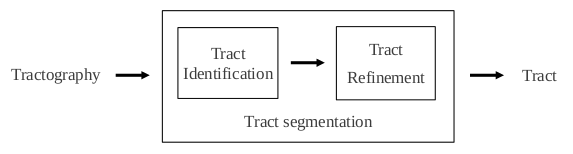
\includegraphics[width=12.5cm, height=2.5cm ]{figures/segmentation.png}
  \caption{A process design of segmentation task, including two steps: tract identification and tract refinement. The tract identification creates the candidate of segmentation from a repository of examples using a supervised algorithm. The candidate then will be refined by experts with the help of the fast clustering technique.}
  \label{fig:ov_tool}
\end{figure*}
The drawback of these approaches is that or they work on a large number of tracks and most of them are not interested to medical practitioners; or they focus on a target tract but the variance between brains makes it difficult to generate well. The results from both case are needed the refinement from expert. In this work, we want to combine both supervised and unsupervised approach to overcome these disadvantage. Moreover, we propose a framework using \textbf{BOI}(Bundles of Interest). While ROI concerns about which streamlines go through some interesting regions, BOI focuses only on streamlines inside some specific bundles. Because all of the current approaches only work on the tracks without caring the anatomy,
% (for example\cite{wakana2007reproducibility} based on ROI-region of interest,~\cite{odonnell2007automatic} needed an Atlas),
and it makes difficult to validate the result. Using BOI would make medical practitioners concentrate on which tracts they are working on, and of course these tracts also correlate to the anatomy. Moreover, while all the current methods are off-line and medical practitioners can not interact or modify the result of segmentation, in this project, we want to build a tool that can help them instantly to refine the segmentation result mannualy. It is also another novelty of our approach. Beside, this tool should has ability of real time adapting to the responding of users. This is also the other different of our method to most of the state-of-the-art approaches, which can not adjust to the user feedback. In another way, in this project, our goals are to:
%The most challenge is to design a clustering algorithm based on a specific distance function and this algorithm must be effective and real time adaptive to the responding of users. This is also the other different of our method to most of the state-of-the-art approaches, which can not adjust to the user feedback.
%In this project, our goal is to address the segmentation problem based on the BOI (Bundle of Interest) contrasting with ROI (Region of Interest). : 
%What is the outline of research?
\begin{itemize}
	\item First, design an effective method for tract segmentation task using \emph{machine learning} based on BOI approach.
%techniques
	\item Second, develop a scientific interactive visualization tool, which is the implementation of the framework that we propose for tract segmentation task in the previous step.%in the first goal, to help medical practitioners to perform this segmentation task more precisely and easily based on BOI approach.
\end{itemize}
With the assistance of this scientific interactive tool, we have a strong belief that the task of tract segmentation would be done more precisely, more easily and would consume less time.
%This research is motivated to help medical practitioners to do the task of segmentation tractography more easily and accurately. Results of tract segmentation are immediately applicable to surgical intervention, to the design of medical interventions and to the treatment of psychological and psychiatric disorders. The end users who got benefit from this work are patients who have problem with their brain or other cognitive issues.
%We propose a design of interactive segmentation process based on two steps: tract identification 
%based on supervised learning 
%and tract refinement (figure \ref{fig:ov_tool}).
%with the help from unsupervised learning. 
%The tract identification step generates the first hypothesis of segmentation instead of starting from the whole tractography. This step uses the manual segmentation examples from experts to create the candidate of tract segmentation, and we conceive it as a supervised learning task. This step can be solved based on the most recent method introduced in% by Olivetti
%~\cite{olivetti2011supervised}. The next refinement step aims to refine the hypothesis of segmentation and takes place by excluding some unnecessary streamlines or selecting additional ones. With the aim to help medical practitioners to perform this refinement task more precisely and easily, it is necessary to cluster streamlines with similar spatial and shape characteristics into one set, called \emph{bundle}. We design it as a clustering problem, and our main investigation focuses on it.
%In this work we propose to address the \textbf{online segmentation task} by using both \textbf{supervised and unsupervised segmentation} (fast clustering technique). For better using and supporting doctors/neural scientists to do the segmentation task more easy and faster, we build up an interaction visualization tool, call Spaghetti. In this software, there are two main steps: the first step uses supervised learning to make the candidate of segmentation from the repository of examples. Then, doctors/neural scientists will refine this candidate in the next step with the help from fast clustering technique. The frame work of this software is described in the figure \ref{fig:ov_tool}. After the segmentation task, the result is then used for some clinical diagnosis applications.
%In this work we propose to address the segmentation tractography task as both unsupervised and supervised segmentation problem based on dissimilarity approximation. 
%Brain connectivity analysis methods – joint modeling of structural and functional brain connectivity, relationship between structural and functional connectivity, and dynamics of connectivity. more infor at http://mbia2012.web.unc.edu/
%Another one is leverage the expert-crafted streamline-streamline distance functions available from the literature and to use them in a dissimilarity based~\cite{pekalska2002generalized} representation of the problem. It means that instead of working directly to tractography dataset as these past approaches, we try to propose a new representation space for the tractography based on dissimilarity approximation. Moreover we note that the widely adopted kernel-based classification algorithms cannot directly embed such distance functions into a kernel because the kernel would violate the necessary assumption of being positive semi-definite~\cite{pekalska2002generalized,chen2009similarity}. Due to that, it is necessary to vectorize the tractography in the standard space before applying current novel learning techniques to segment. We believe that with this vectorizing, the segmentation tractography task using both unsupervised and supervised learning will get the novel results.
%of\footnote{A fourth, and last, footnote.}






%%ACKNOWLEDGMENTS are optional
\section{Problem statement}
\label{sec:problem_statement}
\textbf{\textit{Basic notation:}} Let the polyline $s =\{ \vec{x_1},\ldots,\vec{x}_{n_s}\}$, where $\vec{x} \in \mathbb{R}^3$, be a \emph{streamline} reconstructed from dMRI data by deterministic tractography algorithms~\cite{mori2002fiber}. Let the \emph{tractography} $ \mathbb{T}  = \{s_1,\ldots,s_n\}$ be defined as a set of $n$ streamlines. 
%We assume that $\mathbb{T}$ is sampled according to a probability distribution $\mathfrak{T}$ which incorporates the variance of data related to the dMRI measurement process and the variability of subjects. %Current dMRI techniques operated on adult humans generate tractography of size in the order of $3 \times 10^5$ streamlines. 
Let $\tau$ be an anatomical fiber tract of interest, e.g. the cortical spinal tract (see figure~\ref{fig:CST}), and let $\mathsf {T} \subset \mathbb{T}$ be its corresponding streamline-based approximation within given the tractography.

\textbf{\textit{Process design:}} we propose a design of interactive segmentation process based on two steps(figure \ref{fig:ov_tool}): tract identification based on supervised learning and tract refinement based on unsupervised learning.
The \emph{tract identification step} generates the first hypothesis of segmentation instead of starting from the whole tractography. It uses the manual segmentation examples from experts to create the candidate of tract segmentation.  The tract identification step  corresponds to a mapping $f : \mathbb{T} \mapsto \{0,1\}$ where
\begin{equation}
\label{eq:neuroanatomist_f}
f(s) =
\left\{
  \begin{array}{rl}
    1 & \mbox{if } s \mbox{ in } \mathsf{T} \\
    0 & \mbox{otherwise}
  \end{array}
\right.
\end{equation}
In the machine learning terminology, the function $f$ is called \emph{classifier} and each pair $(s,f(s))$ is a class-labeled
\emph{example}. In practice $f$ is not available % in algorithmic form
and the problem is then to infer an approximation $g$ from data. We
may have many samples of $\mathsf{T}$ for the same fiber tract $\tau$, e.g. the
cortical spinal tract, when the annotation is operated by different neuroanatomists. The labelling is prone to error and has to be considered an approximation of the true fiber tract. A classifier $g$ is learned by training a classification
algorithm from the set $\mathsf{T}$.
% $A$ which optimize a loss function $L$. 
%Common classification algorithms are the $k$-nearest neighbor ($k$NN)~\cite{devroye1996probabilistic} and the Support Vector Machines (SVMs)~\cite{boser1992training}. A usual loss function is the $0-1$ loss $L(s,g(s)=I(s,g(s))$ where $I$ is the indicator function.
Detail about supervised classifier for tractography can be found in~\cite{olivetti2011supervised}. Our main focus in this project is not on this step, but on the next step.

%\subsection{\textbf{Analytic definition of problem}}
%Formal definition of clustering problem
Let $\mathcal{T} \subset \mathbb{T}$ and $\mathcal{T} =\{ \mbox{s  } \mid \mbox{ } g(s)=1, \forall s \in \mathbb{T} \}$. In an ideal case, $\mathcal{T} \equiv \mathsf{T}$, but it rarely happens due to the error of function $g(s)$ during the training stage.
The \emph{tract refinement step} aims at refining the $\mathcal{T}$ for being close to the $\mathsf{T}$ by excluding any unnecessary streamlines or selecting additional ones. In contrast to the previous step, which automatically done by learning from a repository of examples, this refinement step is manually performed by medical practitioners. When they do the segmentation, it is often an important requirement of viewing $\mathcal{T}$ at different levels of grouping for better visualization in detail.
%. Medical practitioners usually changes between these levels for better visualization. 
This demand raises a question of how to present $\mathcal{T}$ in different level of abstraction. This requirement is much stricter than randomly sampling representatives of $\mathcal{T}$ and hiding the others. In another way, we need a clustering algorithm which has a capability of producing different partitions of $\mathcal{T}$ corresponding to different levels of viewing. We consider it as an unsupervised learning problem. 

\textbf{\textit{Data representation:}}
%The efficiency structure for representation, storing and accessing data:}}
However, most of the state-of-the-art learning techniques (both supervised and unsupervised) 
%in order to calculate the (dis)similarity bewteen two items, this method (also other state-of-the-art clustering approaches)
often require the data to lie in a vectorial space, which is not the case of streamlines. Streamlines are polylines in $3$D space. Each streamline $s =\{ \vec{x_1},\ldots,\vec{x}_{n_s}\}$, where $\vec{x} \in \mathbb{R}^3$, has different length and different number of points, and for this reason they cannot be directly represented in a common vectorial. The lack of the vectorial representation avoids the use of some of these algorithms and of computationally efficient implementations. In this case, we need to find a representation $\phi$ of streamline in a vectorial space $\phi : \mathbb{T} \mapsto \mathbb{R}^d$, where $d$ is the dimension of the new space. This representation $\phi$ maps a streamline $s$ from its original space $\mathbb{T}$ to a
vector of $\mathbb{R}^d$. This representation is a \emph{lossy} one in the sense that in general it is not possible to exactly reconstruct $s$ from $\phi(s)$ because some information is lost during the projection. How we can minimize this \emph{lossy} is really a challenge. 
%Each streamline$s =\{ \vec{x_1},\ldots,\vec{x}_{n_s}\}$, where $\vec{x} \in \mathbb{R}^3$, has different length and different number of points and for this reason they cannot be directly represented in a common vectorial space, which is the input requirement of most of the current machine learning algorithms. In this work, it is our duty to propose a method for representing streamline in another space with the same dimension. 
Beside, due to the huge number streamlines, the number of partitions and clusters are also very large. It makes storing and accessing partitions and clusters hard and resource consuming. Therefore, an efficiency structure for representation, storing and accessing clusters and partitions is another important requirement which needs to be fulfilled.
\\After projecting streamlines into a vectorial space $\mathbb{R}^d$ by using an efficient representation $\phi$, the next step is how we can cluster streamlines (in representation space $\phi(s)$) into different clusters corresponding to different levels of viewing.% from users. 
In the following part, we will first present the formal definition of clustering problem, and then state the problem of tractography clustering.
%The simplest way is to re-run the clustering algorithm whenever the experts change the level of viewing. But this will consume a lot of time and cost computation a lot. In this part, we will first present the formal definition of clustering problem, and then state the task of tractography clustering. 
%In the general view, from this point to end, it is possible to consider $\mathcal{T}$ as an N-streamline \textit{tractography} $ \mathcal{T}  = \{s_1,\ldots,s_N\}$.
%And our task is to provide an interaction visualization tool to help them to do this task more easily and more accurately.

\textbf{\textit{Clustering problem:}} Clustering is a division of data (or data representation) into a certain number of clusters (groups, subsets, or categories). Up to present, the definition of clustering has still not been agreed universally. Most researchers describe a cluster by considering the internal homogeneity and the external separation, i.e., the similarity between objects within a subgroup is larger than the similarity between objects belonging to different subgroups. Both the similarity and the dissimilarity should be defined in a clear and meaningful way. Here, we give some simple mathematical descriptions of several types of clustering, based on the description in~\cite{xu2005survey}.
\\Given a set of input patterns denoted as $\mathcal{X} = \{\mathsf{x_1}, \ldots, \mathsf{x_j}, \ldots, \mathsf{x_N}\}$ where $\mathsf{x_j} = (x_{j1},x_{j2}, \ldots,x_{jd})^T \in \mathfrak{R}^d$ and each measure $x_{ji}$ is said to be a feature (attribute, dimension, or variable).
Clustering attempts to seek a $K$-partition of $\mathcal{X}$, $C = \{C_{1}, \ldots, C_{K}\}$, with $K \leq N$, such that
\begin{equation}
\label{clustering_condition}
C_{i}\neq \varnothing, \textit{i = 1, \ldots, K} \mbox{  and  } \cup_{i=1}^{\textit{K}}C_{i} = \mathcal{X}
\end{equation}
%\begin{equation}
%\label{condition1_cluster}
%\cup_{i=1}^{\textit{K}}C_{i} = \mathcal{X}
%\end{equation}
%\begin{enumerate}
%	\item	$C_{i}\neq \varnothing, \textit{i = 1, \ldots, K}$
%	\item $\cup_{i=1}^{\textit{K}}C_{i} = \mathcal{X}$
%	\label{clustering_condition}
%\end{enumerate}
The difference of the definition of the separation between clusters leads to different types of clustering.
%\begin{itemize}
%	\item 
\textit{Hard partitional clustering} accepts no overlaping between partitions. All clusters are exclusive, so that each patterns only belongs to one cluster
	$C_{i} \cap C_{j} = \varnothing$, $i,j = \textit{1, \ldots, K}$, and $i \neq j$.
%	\item 
\textit{Hierarchical clustering} tries to construct a tree-like nested structure partition of $\mathcal{X}$:	
	$H = \{H_{1}, \ldots, H_{Q}\}$, with $Q \leq N$, such that $C_{i} \in H_{m}, C_{j} \in H_{l}, m > l$ 	
	imply  $C_{i} \in C_{j}$ or $C_{i} \cap C_{j} = \varnothing$, for all $i,j \neq i, m, l = 1, \ldots, Q$.
%	\item 
\textit{Fuzzy clustering} allows one pattern to belong to all clusters with a degree of membership, $\mu_{i,j} \in [0,1]$, which represents the membership coefficient of the $j$th object in the $i$th cluster and satisfies the following two constraints:
	$\sum_{i=1}^{K} \mu_{i,j} = 1,  \forall j$ and $\sum_{j=1}^{N} \mu_{i,j} \leq N, \forall i$
%\end{itemize} 

\textbf{\textit{Distance and similarity:}}
It is natural to ask what kind of standards we should use to determine the closeness, or how to measure the distance (dissimilarity) or similarity between a pair of objects, an object and a cluster, or a pair of clusters. A data object is described by a set of features, usually represented as a multidimensional vector. 
%The features can be quantitative or qualitative, continuous or binary, nominal or ordinal, which determine the corresponding measure mechanisms. 
\\A distance or dissimilarity function on a data set $\mathcal{X}$ between individuals is defined to satisfy the following conditions.
\begin{equation}
     (d(\mathsf{x_i},\mathsf{x_j}) = d(\mathsf{x_j},\mathsf{x_i})) 
     \wedge
     (d(\mathsf{x_i},\mathsf{x_j}) \geq 0), \forall \mathsf{x_j},\mathsf{x_i}
\end{equation}
if two following conditions (triangle inequality~\ref{distance_triangle_ineuqality} and reflexity~\ref{distance_reflexity}) are still hold, the distance is called a metric
\begin{equation}
     d(\mathsf{x_i},\mathsf{x_k}) + d(\mathsf{x_k},\mathsf{x_j}) \geq d(\mathsf{x_i},\mathsf{x_j}), 
     \forall \mathsf{x_i},\forall\mathsf{x_j},\forall\mathsf{x_k}
     \label{distance_triangle_ineuqality}
\end{equation}
\begin{equation}
     d(\mathsf{x_i},\mathsf{x_j}) = 0 \leftrightarrow \mathsf{x_j}\equiv \mathsf{x_i} 
     \label{distance_reflexity}
\end{equation}
Likewise, a similarity function is defined to satisfy the conditions in the following.
\begin{equation}
     (s(\mathsf{x_i},\mathsf{x_j}) = s(\mathsf{x_j},\mathsf{x_i})) 
     \wedge
     (0 \leq s(\mathsf{x_i},\mathsf{x_j}) \leq 1), \forall \mathsf{x_j},\mathsf{x_i}
\end{equation}
if two following conditions are still satisfied, it is called a similarity metric
\begin{equation}
     [s(\mathsf{x_i},\mathsf{x_k}) + s(\mathsf{x_k},\mathsf{x_j})]s(\mathsf{x_i},\mathsf{x_j}) \geq s(\mathsf{x_i},\mathsf{x_k})s(\mathsf{x_k},\mathsf{x_j}), 
     \forall \mathsf{x_i},\mathsf{x_j},\mathsf{x_k}
\end{equation}
\begin{equation}
     s(\mathsf{x_i},\mathsf{x_j}) = 1 \leftrightarrow \mathsf{x_j}\equiv \mathsf{x_i} 
\end{equation}
Based on the definition (dis)similarity between two objects, there are many way to define the (dis)similarity between a object and a cluster, or a pair of clusters. A popular group of distances is the modified Hausdorff distances~\cite{dubuisson1994modified}. See~\cite{zhang2008identifying} for a recent survey about these distances. 
\\For a data set with $N$ input patterns, we can define an $N \times N$ symmetric matrix, called proximity matrix, whose $(i,j)$th element represents the (dis)similarity measure for the $i$th and $j$th patterns $(i,j = 1, \ldots, N)$. Obviously, the (dis)similarity measure directly affects the formation of the resulting clusters. Almost all clustering algorithms are explicitly
or implicitly connected to some definition of proximity measure. Some algorithms even work directly on the proximity matrix. Once
a proximity measure is chosen, the construction of a clustering criterion function makes the partition of clusters an optimization problem, which is well defined mathematically, and has rich solutions in the literature. The survey of clustering algorithms and distance functions can be found in~\cite{xu2005survey, rai2010survey}. Different approaches usually lead to different clusters; and even for the same algorithm, parameter identification or the presentation order of input patterns may affect the final results. Therefore, it is important to carefully investigate the characteristics of the problem at hand, in order to select or design an appropriate clustering strategy.
 %Most of clustering algorithms often rely on distance functions, then followed by a clustering algorithm (agglomerative, k-means, Gaussian mixture model, etc. see~\cite{xu2005survey, rai2010survey} for a recent brief review). 

%\subsection{\textbf{What we want to do: clustering tractography}}
\textbf{\textit{Clustering tractography}}
Given a set of $N$ streamlines $ \mathcal{T}  = \{s_1,\ldots,s_N\}$~\footnote{note that $s_i, \forall i \in [1, .., N]$ 
is the representation of the original streamline $s_{i}^{'}$ through a representation method $\phi$: $s_i = \phi(s_{i}^{'})$},
traditional approaches for clustering tractography usually find a partition $C = \{C_{1}, \ldots, C_{K}\}$ with $K \leq N$, satisfying two conditions of clustering~\ref{clustering_condition} $C_{i}\neq \varnothing, \textit{i = 1, \ldots, K}$ and $\cup_{i=1}^{\textit{K}}C_{i} = \mathcal{T}$ (see more in section~\ref{sec:state_of_the_art}). However, in this work, as declared before, we want to seek not only one partition but instead, a set $m$ partitions of a $\mathcal{T}$: $\mathbb{P} = \{P_{1}, P_{2}, \ldots, P_{m}\}$, where $P_{i} = \{C_{1}^{i}, C_{2}^{i}, \ldots, C_{d_{i}}^{i}\}$ is one partition of $\mathcal{T}$ ($d_{i}$ is the number of clusters in partition $P_{i}$). Each partition $P_i$ represents for the $i$th level of abstraction of $\mathcal{T}$. Obviously, within one partition $P_{i}$, there is no intersection between two clusters: $C_{k}^{i} \cap C_{l}^{i} = \varnothing$, with $\forall k,i \in [1,\ldots, d_{i}], k \neq i$. But it is allowed to overlap between one cluster belonging to one partition with another cluster of the other partition:
\begin{equation}
\label{eq:condition_clusters}
 (C_{k}^{i} \cap C_{l}^{j} = \varnothing) \vee (C_{k}^{i} \cap C_{l}^{j} \neq \varnothing), \forall i,j \in [1, .., m], i \neq j  
\end{equation}
The simplest way to solve this problem is to run $m$ times one current clustering algorithm. But take in to account that the number of streamlines is really huge, and most of clustering algorithms often need to calculate pairwise distances of size $N \times N$ where $N$ is the number of tracks. This amount of comparisons puts a massive load on clustering algorithms forcing them to be inefficient and therefore impractical for our purpose. 
Beside, partitions of $\mathbb{P}$ are not unrelated to each other at all. Supposed that the abstraction of the $i$th level is higher than $j$th level. 
%Another reason is that, although there is no explicit rule about constrain between the partition $P_i$ and $P_j$($i,j \in [1, .., m]$), but it dose not mean that there is no relationship between $P_i$ and $P_j$. Because 
Let $P_i$ and $P_j$ represent for the level of abstraction $i$th and $j$th respectively. Then the relationship between clusters $C_{l}^{i} \in P_i$ and $C_{k}^{j} \in P_j$ can be presented as: 
\begin{equation}
\label{eq:parttition_ij}
%	\forall  P_i, P_j, i \geq j \longmapsto \exists C_{k}^{i}:  C_{k}^{i} \in P_j, k \in [1, \ldots, d_i]   
	\forall  P_i, P_j, i \geq j \mapsto [(C_{k}^{j} \subset C_{l}^{i}) \vee (C_{k}^{j} \cap  C_{l}^{i} = \emptyset)]    
\end{equation}
with $l \in [1, \ldots, d_i],k \in [1, \ldots, d_j]$. The most challenge is to design a clustering algorithm, based on a specific distance function, which is able to create a set of $m$-partition $\mathbb{P}$ of $\mathcal{T}$, which satisfies condition~\ref{eq:parttition_ij}. 
%This character would be effective in real time adapting to the responding of users. 
It makes our method different to most of the state-of-the-art approaches~\cite{wakana2007reproducibility,odonnell2007automatic}, which can produce only one partition of $\mathcal{T}$.
%, which can not adjust to the user feedback. 
%Involving to this algorithm, there are also many related issues we have to take into account, such as how we can decide the number of partitions $m$? For each partition $P_i$, what is the number of cluster $d_i$? What is the strategy for initializing clusters? Which function we use to measure the (dis)similarity?% between a pair of streamlines, a streamline and a cluster, or a pair of clusters? 
%The drawback of these approaches is to work on a large number of tracks and most of them are not interested to the medical experts. Another disadvantage is that all the tracks are not related to the anatomic (for example\cite{wakana2007reproducibility} based on ROI-region of interest,~\cite{odonnell2007automatic} needed an Atlas), and it makes difficult to validate the result. In contrast with them, in this project, we propose a framework using \textbf{BOI}(Bundles of Interest), which focuses on the group of interesting tracks, and of course it also based on the anatomy. Moreover, while all the current methods are off-line and medical practitioners can not interact or modify the result of segmentation, in this project, we want to build a tool that can help them instantly to adjust the segmentation result. It is also another novelty of our approach. The most challenge is to design a clustering algorithm based on a specific distance function and this algorithm must be effective and real time adaptive to the responding of users. This is also the other different of our method to most of the state-of-the-art approaches, which can not adjust to the user feedback.

%Up to present, only Hierarchal clustering~\cite{johnson1967hierarchical} has a capability of producing a structure of clusters, while all of the other current methods only have result of one partition.
Another raising problem is that, when medical practitioners do the segmentation, eventhough they do select some clusters, they also want to \textit{check} that some neighbor streamlines \textit{"close"} to these clusters should be included into or excluded from the result or not (called \textit{neighbor checking} problem). Let $P_{i} = \{C_{1}^{i}, C_{2}^{i}, \ldots, C_{d_{i}}^{i}\}$ be the current viewing partition of $\mathcal{T}$, and $\mathcal{T}_{s}$ be the set of $m$-selected streamlines $ \mathcal{T}_s  = \{s_1^s,\ldots,s_m^s\}$. At the beginning, $\mathcal{T}_s = \bigcup_{j=1}^{d_i} C_j^i = \mathcal{T}$. % (in the later steps the first condition is not satisfied). %, there is no requirement of $\mathcal{T}_s = \{s_k,\mbox{ } \forall s_k \in C_j^i, \mbox{ } j \in [1,\ldots,d_{i}] \}$. 
Given a distance threshold $\theta$, let $\mathit{neighbor}(s,\theta)$ be a set of close streamlines of streamline $s$. 
\begin{equation}
\label{eq:neighbor_s}
\mathit{neighbor}(s,\theta) = \{s_i \mbox{ |  }d(s,s_i) \leq \theta \mbox{ } \wedge s_i \neq s, \mbox{  }\forall s_i \in \mathbb{T} \}
\end{equation}
where $d(s_i,s_j)$ is a distance function between $s_i$, $s_j$; and $\mathbb{T}$ is the whole brain tractography. With a streamline set $S$, neighbor of $S$ is defined as $\mathit{neighbor}(S,\theta) = \bigcup_{s_i \in S}\mathit{neighbor}(s_i,\theta)$.
%$\{\mathit{neighbor}(s_i), \mbox{ }\forall s_i \in S\}$. And neighbor of a   If they do choose additional neighbor streamlines, the  which somehow meets our requirement. 
\\\textit{Removing streamline:} Let streamline $s_{rm} \in C_{j}^{i} $ be removed from $\mathcal{T}_{s}$. In this case, only cluster $C_{j}^{i}$ is affected and there is no significant change on $\mathbb{P}$:
\begin{equation}
\label{eq:remove_s}
C_{j}^{k} = C_{j}^{k} \setminus \{ s_{rm}\} \mbox{, if } C_{j}^{k} =\emptyset \mbox{ then }  P_{k} = P_{k} \setminus C_{j}^{i}, \forall k \in [i,..,m]
\end{equation}
%Assuming that after being removed, one streamline could not be re-selected. Under this assumption, every time. 
\textit{Adding streamline:} Supposed streamline $s_{add} \in \mathit{neighbor}(\mathcal{T}_{s},\theta)$ is additionally selected. The new selected set is $\mathcal{T}_{s}^{'} = \mathcal{T}_{s} \cup \{s_{add}\}$ and new partition of $\mathcal{T}_{s}^{'}$ be $P_{i}^{'}$.
Let $\mathbb{P}^{'}$ be the new $m$-partition set of $\mathcal{T}_{s}^{'}$: $\mathbb{P^{'}} = \{P_{1}^{'}, P_{2}^{'}, \ldots, P_{m}^{'}\}$, where $P_{i}^{'}$ is one partition of $\mathcal{T}_{s}^{'}$ at the $ith$ level. 
We consider how to generate $\mathbb{P}^{'}$ from the current $\mathbb{P}$.
Let a triple $<\mathsf{P}, \mathsf{T}, \gamma>$ denote for the partition set $\mathsf{P}$ generated from a set of streamlines $\mathsf{T}$ according to some constraints in $\gamma$. It is clear that $\mathbb{P}$ is generated on $\mathcal{T}$ only based on the constrain $\gamma_1$ of equation~\ref{eq:parttition_ij}: $<\mathbb{P}, \mathcal{T}, \gamma_1>$.

Let $d(s,C)$ be the distance between a streamline $s$ and a cluster $C$. Let $d(C_{i}, C_{j})$ be the distance between two clusters $C_i$ and $C_j$. Let $d(C_{j}^{i},P_{i})$ be the min distance between cluster $C_{j}^{i} \in P_{i}$ with all the other clusters of partition $P_{i}$: 
\begin{equation}
\label{eq:min_dis_cluster}
d(C_{j}^{i},P_{i}) = min_{k\in [1,..d_{i}], k \neq j}(d(C_{j}^{i},C_{k}^{i}))
\end{equation}
Let $C_{close}(s,P_i)$ be the cluster in $P_i$ closest to streamline $s$: 
\begin{equation}
\label{eq:closest_streamline_cluster}
C_{close}(s,P_{i}) = argmin_{\forall C_{l}^{i} \in P_{i}}(d(s,C_{l}^{i}))
\end{equation}
If $d(s_{add}, C_{close}(s_{add},P_{i})) > d(C_{close}(s_{add},P_{i}),P_{i})$, obviously $s_{add}$ would become a new cluster in partition $P_{i}^{'}$: $P_{i}^{'} = P_{i} \cup \{s_{add}\}$.
In this case, $\mathbb{P}^{'}$ is generated from $\mathbb{P}$, with the constraint $\gamma_2$: $<\mathbb{P}^{'}, \mathcal{T}_{s}^{'}, \gamma_2>$, where   $\gamma_2$ is the condition of that all the partitions of $\mathbb{P}^{'}$ lower than $i$th level must be contain $\{s_{add}\}$ as a separative cluster: 
\begin{equation}
\label{eq:separate_cluster}
	\forall j \in [1,..,i], \mbox{ } \exists {C'}_{l}^{j} \in P_{j}^{'}: {C'}_{l}^{j} = \{s_{add}\}
\end{equation}
If $d(s_{add}, C_{close}(s_{add},P_{i})) \leq d(C_{close}(s_{add},P_{i}),P_{i})$, then it is clear that $s_{add}$ would be merged into the cluster $C_{close}(s_{add},P_{i})$: $C_{close}(s_{add},P_{i}) = C_{close}(s_{add},P_{i}) \cup \{s_{add}\}$. In another word, $s_{add}$ and $C_{close}^{i}(s_{add})$ must be in the same cluster from the $ith$ level of abstraction.
For that reason, 
%$s_{add}$ and $C_{close}^{i}(s_{add})$ must be in the same cluster from the $(i+1)th$ level of abstraction,    Obviously, medical practitioners, with their experience, want to group $s_{add}$ and $C_{close}^{i}(s_{add})$ in the same cluster after the $ith$ level of abstraction. 
the set of partitions $\mathbb{P}^{'}$ of $\mathcal{T}_{s}^{'}$ is driven from $\mathbb{P}$: $<\mathbb{P}^{'}, \mathcal{T}_{s}^{'}, \gamma_3>$, with constrain $\gamma_3$:
\begin{equation}
\label{eq:constrain_new_partition}
\forall k \in [i,..,m],\exists C_{j}^{k} \in P_{k}^{'}:(C_{close}(s_{add},P_{i}) \cup \{s_{add}\})\subseteq C_{j}^{k}  
\end{equation}
%In the easy case that $s_{add} \in \mathcal{T}$, then $P_{i}^{'} = P_{i}$. Other while, if $s_{add} \notin \mathcal{T}$, the question is which $C_j^i \in P_{i}$ that $s_{add}$ should belong to? Or it is necessary to create a new cluster $C_{d_{i}+1}^i$? 
%How we can generate $P_{i}^{'}$ from $P_{i}$ is one of the most difficult challenge. 
%Moreover, because $P_i$ is an element of an ordered set of partitions $\mathbb{P}$ (as condition~\ref{eq:parttition_ij}), it makes the determining the place of the new element $s_{add}$ do affect not only on $P_i$ but also on other partitions of $\mathbb{P}$.
%~\cite{ widyantoro2002incremental, wang2010document,ribert1999incremental  }
%the hierarchyhow to an o structure 


%there is no approach addressing this problem. All of the most state-of-the-art methods only produce the result of one partition (except for hierarchal clustering). But for the sake of the end users (doctors, medical practitioners), the requirement of having a set $m$ partitions of $\mathcal{T}$ is necessary and useful. Because we are the first one stating this problem, we also have to face with many challenges as following:
%\begin{itemize}
%	\item \textbf{\textit{A robust clustering algorithm creating $m$ partitions of $\mathcal{T}$:}} 
%	\item
% 	\item\textbf{\textit{Neighbor checking:}} This challenge original comes from the need of practical activity. When doctors or experts do the segmentation, although they do select one  cluster, they also want to \textit{check} that some neighborhood streamlines \textit{"close"} to that cluster should be included into the result or not. All of the state-of-the-art clustering algorithms do not allow to add more object into a cluster after clustering. If we can provide this function for experts, then the task of segmentation would be done more easily and accurately.      
%\end{itemize} 
%\begin{equation}
%\label{eq:neuroanatomist_f}
%f(s) =
%\left\{
%  \begin{array}{rl}
%    1 & \mbox{if } s \mbox{ in } t \\
%    0 & \mbox{otherwise}
%  \end{array}
%\right.
%\end{equation}
%\textbf{The novelty of our work compared with related works}
%Recently there are many approaches to solve the tractography clustering. In~\cite{savadjiev2008streamline}, Savadjiev et. al clustered diffusion orientation distribution functions maxima instead of clustering fiber tracts directly. This algorithm based on the geometric coherence of fiber orientations is proposed. Maddah et al. in~\cite{maddah2008modeling} proposed a probabilistic approach to cluster fibers. There is no need to computing pairwise distances in this approach, because it uses a Dirichlet distribution as a prior to incorporate anatomical information. It used a parametric model, assuming that the number of clusters is known and required manual initialization of cluster centers. This algorithm also required establishing point correspondence which was difficult to define. Wang et al.~\cite{wang2011tractography} proposed a non-parametric Bayesian framework to cluster white matter fiber tracts into bundles using a hierarchical Dirichlet processes mixture (HDPM) model. After the models of bundles is learned from training data without supervision, they can be used as prior to cluster fibers of new subjects for comparison across subjects. This approach does not require computing pairwise distances between fibers, and the number of clusters is automatically learned driven by data with Dirichlet process prior instead of being manually specified.
 %Recently, there is a rise of applying pattern recognition techniques to solve this problem. 
%More precisely, following are what we want to investigate in this project:
%\begin{enumerate}
%\item \textbf{Multimodal brain image visualization:} 
%visualization of large-volume, dynamical multimodal brain image data. A novel contribution of this work is to build up an online interaction visualization software that help doctors/neuro scientists to do the segmentation task easier, faster and instantly.\\
%This tool is the implementation of the step segmentation in the figure \ref{fig:ov_research}. The input of this software is the whole brain tractography plus the repository of manual segmentation examples. The out put is the segmentation after refining by doctors/neural scientists. To help user can use it friendly, easily, beside the main functions (select/deselect bundle, explore bundle, move/hide slice,etc...) some other common tasks should be integrated such as undo, save current work, load the previous work, etc.
%\item \textbf{Brain tractography segmentation:} to do the segmentation of the tractography, in this work, we use both \textit{unsupervised} and \textit{supervised} learning. The reason why using both of them is that each technique is suitable for different steps in the whole process (see more detail about two steps in the figure \ref{fig:ov_tool}. First, supervised learning is used in the hypo generation stage to create the candidate of segmentation. Then, this candidate is refined by doctors/neural scientists based on a fast clustering technique.% to help them interact with tracts easier and faster.
%\par{}
%%\textbf{How we can do this?} 
%\textbf{\textit{Supervised tract segmentation:%Multimodal brain image pattern classification methods}} to classify brain tractography into a specific group using supervised learning technique. The idea of the supervised learning is to exploit examples of manually segmented tracts to learn how to extract them automatically from new subjects. This motivation raises from working with doctors and neuroscientists who have already collected many segmented tractogarphy data but it is very difficult for them to use the knowledge in this data for segmentation the new brain. With supervised learning technique, firstly it is necessary to collect enough the manually segmented tractography data. After that, a system will automatic extract some common features from this dataset. These features will be put into a classifier kernel as the standard to classify the tracts belong to which segmentation. At the first idea, some useful features could be the size of bundle, the number of tracts, the length of tracts. This method focuses on the potential benefit of adapting the model learnt from one subject to an other subject. 
%\par{}
%\textbf{\textit{Fast clustering:}} 
%in contrast with the supervised learning, the unsupervised method requires no prior knowledge from neuroscientists. Such techniques often rely on expert-crafted streamline-streamline distance functions encoding informative relationships for the segmentation task, then followed by a clustering algorithm (agglomerative, k-means, Gaussian mixture model, etc. see~\cite{wang2011tractography} for a recent brief review). Due to the fact that result of the classification based on supervised learning usually does not satisfy the requirement of the doctors/neural scientists, it is necessary to let them refine the segmentation again with the help of fast clustering technique. 
%After projecting the tractography into a vector space, one algorithm for clustering the projected tractography can be used. 
%The first idea is to use hierarchical clustering techniques. The motivation behind this is that this algorithm does not base on a specific number of cluster centers. It creates the whole clusters in a hierarchical tree, and when users change the number of cluster, the result of different clusters or segmentations will be appeared. This clustering technique do help doctors/neural scientists to do the segmentation refinement task easier, faster and instantly.
%seperate  swe want to cross-validate the result to know which method has the senior advantage for segmentation tractography task. With the unsupervised method, it requires no prior knowledge from neuroscientists. Such techniques often rely on expert-crafted streamline-streamline distance functions encoding informative relationships for the segmentation task, then followed by a clustering algorithm (agglomerative, k-means, Gaussian mixture model, etc. see~\cite{wang2011tractography} for a recent brief review). 
% In the other side, the idea of the supervised learning is to exploit examples of manually segmented tracts to learn how to extract them automatically from new subjects. This motivation raises from working with doctors and neuroscientists who have already collected many segmented tractogarphy data but it is very difficult for them to use the knowledge in this data for segmentation the new brain. The challenge is to design an effective computational supervised learning approach for tract segmentation in contrast to unsupervised approach.\\
%\par{}
%\textbf{\textit{Dissimilarity approximation:}}
%both supervised and unsupervised segmentation method base on machine learning technique which requires the input to be from a vectorial space. This requirement contrasts with the intrinsic nature of the tractography because its basic elements, called streamlines or tracks, have different lengths and different number of points and for this reason they cannot be directly represented in a common vectorial space. This lack of the vectorial representation avoids the use of some of those algorithms and of computationally efficient implementations. The dissimilarity space representation could be the way to provide such a vectorial representation and for this reason it is crucial to assess the currently machine learning techniques. Actually, the dissimilarity representation is an Euclidean embedding technique defined by selecting a set of objects (e.g. a set of streamlines) called \emph{prototypes}, and then by mapping any new object (e.g. any new streamline) to the vector of distances from the prototypes. This representation~\cite{pekalska2002generalized,balcan2008theory,chen2009similarity} is usually presented in the context of classification and clustering problems. More detail about this can be found in the section \ref{subsec:dissimilarity}.
%\item \textbf{Clinical applications:} 
%computer aided diagnosis and follow-up of brain diseases via multimodal images, early diagnosis of brain diseases via multimodal images, and differential diagnosis of brain diseases via multimodal images. At the first stage, we want to find the different between the healthy brains and diseased brains of the patients of the ALS disease (Amyotrophic Lateral Sclerosis)\footnote{\url{http://www.alsa.org/about-als/what-is-als.html}}\\
%\textbf{How we can do this?} \textbf{- clinical diagnosing applications}
%The result of tract segmentation based on fast clustering technique is used for early clinical diagnosis applications. For this purpose, the diagnosing can be evaluated based on a set of quantitative and qualitative criteria. The qualitative evaluation of the tract reconstruction will be only performed by expert neurosurgeons and radiologists. Therefore, in this work, the main focus is the quantitative criteria which provide useful information for diagnosing brain diseases. Some useful quantitative signal can be used such as fiber profile on diffusion parameters (FA - fractional anisotropy, MD - mean diffusion, eigenvalues ($<\lambda_1,\lambda_2,\lambda_3>$)), correlation and absolute profile distance measures, fiber geometry of volumetric overlap, and the Hausdorff distances between bundles. These parameters are hints for diagnosing some brain diseases, and we here focus on the ALS (Amytrophy Lateral Smytrophic) disease.
%\end{enumerate}
%\subsection{\textbf{Who: target of this research is for who?}}
%This research is motivated to help medical practitioners to do the task of tractography segmentation more easily and accurately. Results of tract segmentation are immediately applicable to surgical intervention, to the design of medical interventions and to the treatment of psychological and psychiatric disorders. The end users who got benefit from this work are patients who have problem with their brain or other cognitive issues.



%\section{Proposed Solution}
\label{sec:solution}
%Clustering fibers has drawn a lot of attention in recent years and faces many challenges. Full brain tractography typically generates $\approx 3 \times 10^5$ fibers per subject. 
%In some cases, fibers from multiple subjects need to be clustered together for comparison. 
%Thus, the developed algorithms are expected to cluster large scale data sets. Due to data quality and other factors, tractography results may have a significant amount of errors. The clustering algorithms are required to be robust to these errors. 
%In order to compare the fiber bundles of different subjects in group study and save computational cost, it is of interest to explore how to use the fiber bundles learned from old data sets to cluster fibers of new subjects. 
%To obtain fiber bundles which correspond to anatomical structures, the clustering algorithms are expected to related to anatomical information. 
%In this work, we propose to address the segmentation tractography task as both unsupervised and supervised segmentation problem based on dissimilarity approximation. 
%Tractography segmentation has drawn a lot of attention in recent years and faces many challenges. To obtain fiber bundles which correspond to anatomical structures, the segmentation algorithms are expected to incorporate anatomical information input by experts to guide tractography segmentation. 
To fulfill requirements stated in the previous section, in this part, we propose to address the clustering tractography task (described in section~\ref{sec:problem_statement}) as the \textit{hierarchical clustering} based on \textit{dissimilarity approximation}. 
%Our method has these main steps: pre-processing the raw dMRI data to get the tractography in standard format~\cite{bao2012dmri}, presenting the tractography in a vector space using dissimilarity approximation tractography\cite{olivetti2012approximation}, and applying machine learning techniques -\textbf{supervised and fast clustering-unsupervised} to help segmentation the tractography. After that, the segmentation result is applied for ALS disease diagnosis.
\subsection{Dissimilarity approximation for tractography}
\label{subsec:dissimilarity}
%cite the paper of PRNI2012
%After reconstructing the whole tractography of brain, our goal is to cluster these tracks into some specific groups, or segmentation tractography by means of machine learning methods~\cite{zhang2008identifying,wang2011tractography}. 
%Hierarchical clustering seems to be the best solution for our problem. However, 
In order to calculate the (dis)similarity bewteen two items, most of the state-of-the-art clustering approaches requires the data to lie in a vectorial space, which is not the case of streamlines. Streamlines are polylines in $3$D space and have different lengths and numbers of points. The lack of the vectorial representation avoids the use of these algorithms. In this case,
% and of computationally efficient implementations. 
the dissimilarity space representation could be the way to provide such a vectorial representation and for this reason it is crucial to assess the degree of approximation introduced in~\cite{olivetti2012approximation}. 
\begin{figure}
  \centering
  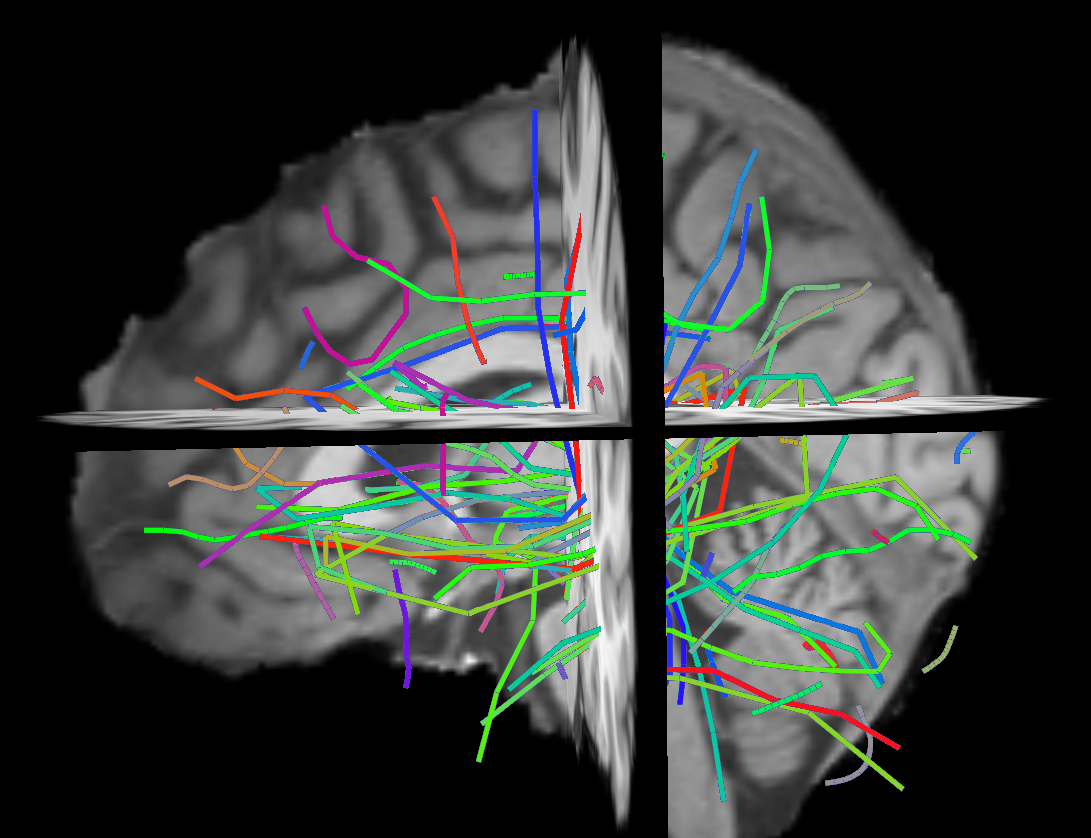
\includegraphics[width=3.2cm]{prni2012b.png}
  \caption{A set of $100$ streamlines, i.e. an example of prototypes, from a full tractography}
  \label{fig:streamlines}
\end{figure}
%copy and paste from the PRNI2012 - need to rewrite

The dissimilarity representation is an Euclidean embedding technique defined by selecting a set of objects (e.g. a set of streamlines) called prototypes, and then mapping any new object (e.g. any new streamline) to the vector of distances from the prototypes. Let have an $N$-streamline set $\mathcal{T} = \{s_1,\ldots,s_N\}$. 
%Let $P_{\mathcal{T}}$ be a probability distribution over $\mathcal{T}$. 
Let $d:\mathcal{T} \times
\mathcal{T} \mapsto \mathbb{R}^+$ be a distance function between two streamlines in $\mathcal{T}$. Note that $d$ is not assumed to be necessarily metric. Let $\Pi = \{\tilde{s}_1, \ldots, \tilde{s}_p\}$, where $\forall i$ $\tilde{s}_i \in \mathcal{\mathcal{T}}$ and $p$ is finite. We call each $\tilde{s}_i$ as \emph{prototype} or \emph{landmark}. The \emph{dissimilarity representation}/\emph{projection} is defined as $\phi_{\Pi}^d(s):\mathcal{\mathcal{T}} \mapsto \mathbb{R}^p$
s.t. 
\begin{equation}
  \phi_{\Pi}^d(s) = [d(s,\tilde{s}_1) ,\ldots, d(s,\tilde{s}_p)]
\label{eq:dissimilarity_representation}
\end{equation}
and maps a streamline $s$ from original space $\mathcal{T}$ to a vector of $\mathbb{R}^p$. 
%Note that this representation is a \emph{lossy} one in the sense that in general it is not possible to exactly reconstruct $X$ from $\phi_{\Pi}^d(X)$ because some information is lost during the projection. 
We define the distance between projected objects as the Euclidean distance between them: $\Delta_{\Pi}^d(s, s') = || \phi_{\Pi}^d(s) - \phi_{\Pi}^d(s') ||_2$, i.e. $\Delta_{\Pi}^d:\mathcal{T} \times \mathcal{T} \mapsto \mathbb{R}^+$. 
%It is intuitive 
Obviously, $\Delta_{\Pi}^d$ and $d$ should be strongly related.
Two main issues of the dissimilarity approximation lie on the strategies to choose prototypes (the number of prototypes and how to choose prototypes) and the measure of approximation to estimate the level of reconstruction $\mathcal{T}$ from $\phi_{\Pi}^d(\mathcal{T})$ (usually called \emph{lossy}). 

The issue of choosing the prototypes in order to achieve the desired degree of approximation usually bases on three popular selection policies: random selection, farthest first traversal (FFT) and subset farthest first (SFF)~\cite{turnbull2005fast}. 
\textit{Random policy} draws uniformly at random from $\mathcal{T}$, i.e. $\Pi \subseteq \mathcal{T}$ and $|\Pi|=p$.
\textit{FFT} selects an initial prototype at random from $\mathcal{T}$ and then each new one is defined as the farthest element of $\mathcal{T}$ from all previously chosen prototypes. 
FFT policy is related to the \emph{$k$-center} problem
%~\cite{hochbaum1985best}
: given a set $S$ and an integer $k$, what is the smallest $\epsilon$ for which you can find an $\epsilon$-cover\footnote{Given a metric space $(\mathcal{X},d)$, for any $\epsilon > 0$, an $\epsilon$-cover of a set $S \subset \mathcal{X}$ is defined to be any set $T \subset S$ such that $d(x,T) \leq \epsilon, \forall x \in S$. Here $d(x,T)$ is the distance from point $x$ to the closest point in set $T$} of $S$ of size $k$? \textit{SFF} policy samples $m = \lceil c p \log p \rceil$ points from $\mathcal{T}$ uniformly at random and then applies FFT on this sample in order to select the $p$ prototypes (c is an constant). All these policies are parametric with respect to the number of prototypes $p$. In the case of tractography, based on our experiments, SFF obtains an efficient and effective selection of the prototypes compared with two other methods~\cite{olivetti2012approximation}.
%As a measure of the degree of approximation of the dissimilarity representation, in the literature of the Euclidean embeddings of metric spaces, the term of \emph{distortion} is usually used~\cite{linial1995geometry}. It represents the relation between the distances in the original space and the corresponding ones in the projected space. 
%The embedding is said to have \emph{distortion}$\leq c$ if for every $x,x' \in \mathcal{X}$:
%\begin{equation}
%  \label{eq:distortion}
%  d(x,x') \geq \Delta_{\Pi}^d(x,x') \geq \frac{1}{c} d(x,x').
%\end{equation}
%Unfortunately this embedding is computationally too expensive to be used in practice. We investigate the relationship between the distribution of distances among objects in $\mathcal{X}$ through $d$ and the corresponding distances in the dissimilarity representation space through $\Delta_{\Pi}^d$. We claim that a good dissimilarity representation must be able to accurately preserve the partial order of the distances, i.e. if $d(X,X') \leq d(X,X'')$ then $\Delta_{\Pi}^d(X,X') \leq \Delta_{\Pi}^d(X,X'')$ for each $X,X',X'' \in \mathcal{X}$ almost always. 
\\As a measure of the degree of approximation of the dissimilarity representation, in the literature of the Euclidean embeddings of metric spaces, the term of \emph{distortion} is usually used~\cite{linial1995geometry}.
It represents the relation between the distances in the original space and 
%the corresponding ones 
in the projected space. 
The embedding is said to have \emph{distortion}$\leq c$ if for every $s,s' \in \mathcal{T}$:
\begin{equation}
  \label{eq:distortion}
  d(s,s') \geq \Delta_{\Pi}^d(s,s') \geq \frac{1}{c} d(s,s').
\end{equation}
However, this embedding is computationally too expensive to be used in practice. We investigate the relationship between the distribution of distances among streamlines in $\mathcal{T}$ through $d$ and the corresponding distances in the dissimilarity representation space through $\Delta_{\Pi}^d$. A good dissimilarity representation must be able to accurately preserve the partial order of the distances, i.e. if $d(s,s') \leq d(s,s'')$ then $\Delta_{\Pi}^d(s,s') \leq \Delta_{\Pi}^d(s,s'')$ for each $s,s',s'' \in \mathcal{T}$. We define the Pearson correlation %coefficient
$\rho$ between the two distances over all possible pairs of streamlines in $\mathcal{T}$:
\begin{equation}
  \label{eq:accuracy_correlation}
  \boldsymbol{\rho} = \frac{\mathrm{Cov}(d(s,s'),
    \Delta_{\Pi}^d(s,s'))}{\sigma_{d(s,s')} \sigma_{\Delta_{\Pi}^d(s,s')}}
\end{equation}
%where $s,s' \sim P_{\}$.  
An accurate correlation coefficient between
objects in $\mathcal{T}$ results in values of $\boldsymbol{\rho}$ far
from zero and close to $1$. The correlation focusses on the
\emph{averaged} differences between the original and projected space
while the distortion cares about the worst case scenario. For this reason, in our case, the correlation is a more appropriate measure. 
%In practical cases $P_X$ is unknown and only a finite sample $S$ is available. We can approximate $\boldsymbol{\rho}$ as the \emph{sample} correlation $\boldsymbol{r}$ where $X,X' \in S$. An accurate approximation of the relative distances between objects in $\mathcal{X}$ results in values of $\boldsymbol{\rho}$ far from zero and close to $1$\footnote{Note that negative correlation is not considered as accurate approximation. Moreover it never occurred during experiments}.

\subsection{Hierarchical clustering}%more on Eletherios thesis page 76
\label{subsec:hierarchical}
%\textbf{Reference more in \cite{schultz2011feature} pages 2 to 5} %thomas2011feature
%In the previous step, we use a set of example of the manual segmentaion to guide the segmentation procedure automatically through supervised learning. But the result of supervised segmentation is usually not satisfactory the requirement of doctors/neural scientists, and it is necessary to refine the segmentation. A clustering of some kind seems to be a solution to provide a useful technique to refine the segmentation. However, most of clustering algorithms return a flat unstructured set of clusters, require a prespecified number of clusters as input and are nondeterministic.  Moreover, most proposed clustering algorithms are very slow and often need to calculate pairwise distances of size $NxN$ where $N$ is the number of tracks. This amount of comparisons puts a massive load on clustering algorithms forcing them to be inefficient and therefore impractical for high frequency using as it is difficult to compute all these distances or even store them in memory. 
Hierarchical clustering~\cite{johnson1967hierarchical} produces a structure of clusters that is more informative than the unstructured set of clusters returned by flat clustering. This characteristic meets the requirement of creating an $m$-partition set $\mathbb{P}$ of $\mathcal{T}$ 
%the immediately responding to the changing level of abstraction of user 
without re-running the clustering algorithm again. Another advantage is that hierarchical clustering does not require to pre-specify the number of clusters. It builds nested clusters by merging them successively, and this hierarchy of clusters represented as a tree (or dendrogram). The root of the tree is the unique cluster that gathers all the samples, the leaves being the clusters with only one sample. In another way, hierarchical clustering algorithm
% (http://scikit-learn.org/stable/modules/clustering.html) 
can clusters data firstly on $N$ centers and consequently until only one center. This main character leads to the capability of visualizing $\mathcal{T}$ in many levels of abstraction, and the users can browse the value of level from $1$ to $N$, to see the clusters immediately.

With an $N$-streamline set $\mathcal{T} = \{s_1,\ldots,s_N\}$, hierarchical produces $Q$ clusters of $\mathcal{T}$
$H = \{H_{1}, \ldots, H_{Q}\}$, with $Q \leq N$, such that $C_{i} \in H_{m}, C_{j} \in H_{l}, m > l$
imply $C_{i} \in C_{j}$ or $C_{i} \cap C_{j} = \varnothing$, for all $i,j \neq i, m, l = 1, \ldots, Q$.
Hierarchical clustering algorithms are either top-down or bottom-up. Bottom-up algorithms treat each streamline as a singleton cluster at the outset and then successively merge (or agglomerate) pairs of clusters until all clusters have been merged into a single cluster that contains all tracts. Bottom-up hierarchical clustering is therefore called Hierarchical Agglomerative Clustering (HAC). Top-down clustering requires a method for splitting a cluster. It proceeds by splitting clusters recursively until individual streamlines are reached \cite{johnson1967hierarchical}.

Given an $N$-streamline set $\mathcal{T}$
%a set $\mathcal{T}$ of $N$ streamlines to be clustered, 
and an $N\times N$ (dis)similarity matrix, the basic process of HAC clustering~\cite{johnson1967hierarchical} is this:
\begin{enumerate}
	\item Assign each streamline to one cluster. We now have $N$ clusters, each containing just one streamline.
	%Let the distances (similarities) between the clusters the same as the distances (similarities) between the items they contain.
	\item Find the closest (most similar) pair of clusters and merge them into a single cluster.
	\item Compute distances (similarities) between the new cluster and each of the old clusters.
	\item Repeat steps $2$ and $3$ until all streamlines are clustered into a single cluster of size $N$.
\end{enumerate}
%$\mbox{   }\mbox{ }1.$ Assign each streamline to one cluster, and have $N$ clusters\\%, each containing just one streamline.\\
%$\mbox{   }\mbox{ }2.$ Find the closest (most similar) pair of clusters and merge\\
%$\mbox{          }$$\mbox{  }$$\mbox{  }$ them into a single cluster.\\
%$\mbox{   }\mbox{ }3.$ Compute distances (similarities) between the new cluster\\ 
%$\mbox{          }\mbox{ }\mbox{ }$ and each of the old clusters.\\
%$\mbox{   }\mbox{ }4.$ Repeat steps $2$ and $3$ until all streamlines are clustered\\
%$\mbox{          }\mbox{ }\mbox{ }$  into a single cluster of size $N$.
%Find the closest (most similar) pair of clusters and merge them into a single cluster, so that now you have one cluster less.
%Compute distances (similarities) between the new cluster and each of the old clusters.
%Repeat steps 2 and 3 until all items are clustered into a single cluster of size N. (*)
Step $3$ can be done in different ways, which distinguishes single-linkage, complete-linkage and average-linkage.
In \emph{single-linkage} clustering (also called the connectedness or minimum method), the distance between a pair of clusters $A$ and $B$ is the shortest distance from any streamline of one cluster to any streamline of the other cluster. 
%If the data consist of similarities, we consider the similarity between one cluster and another cluster to be equal to the greatest similarity from any member of one cluster to any member of the other cluster.
%${d}_sg(A,B) = \min_{i=1,\ldots,n_{s_A}} d({x}_i^A, s_B)$
\begin{equation}
\label{eq:distance_single_linkage}
d(A, B) = \min_{s_A \in {A},s_B \in {B}} d(s_A,s_B)
\end{equation}
where $d(s_A,s_B)$ is the distance between two streamlines:
\begin{equation}
\label{eq:distance_point_streamline}
d(s_A, s_B) = \min_{x_i^A \in s_A, x_j^B \in s_B}||{x}_i^A -{x}_j^B||_2
\end{equation}
with $x_i^A$ and $x_j^B$ are points belonging to streamline $s_A$ and $s_B$ respectively. 
In \emph{complete-linkage} clustering (also called the diameter or maximum method), we consider the distance between cluster $A$ and cluster $B$ to be equal to the greatest distance from any member of one cluster to any member of the other cluster.
\begin{equation}
\label{eq:distance_complete_linkage}
d(A, B) = \max_{s_A \in {A},s_B \in {B}} d(s_A,s_B)
\end{equation}
In \emph{average-linkage} clustering, the distance between two clusters $A$ and $B$ is defined as the average distance from any streamline of cluster $A$ to any streamline of cluster $B$.
\begin{equation}
\label{eq:distance_average_linkage}
d(A, B) = avg_{s_A \in {A},s_B \in {B}} d(s_A,s_B)
\end{equation}
In this project, we use the bottom-up hierarchical clustering (HAC strategy) combining with many distance measurements. The reason it that it is readily available to the fact that at the lowest level of abstraction, all streamlines should be presented, and when user changes the level of abstraction, some of present streamlines would be grouped and replaced by a representative. We hope that the HAC clustering can generate meaningful clusters with minimum memory consumption and respond in seconds with changes from user. However, HAC has not the capability to solve the problem of \emph{neighbor checking}. The solution for this problem is still under the investigation.

%\section{Preliminary results}
\label{sec:preliminary_results}
As described in figure~\ref{fig:ov_tool}, the proposed framework for tract segmentation has two main steps: creating hypo candidate from whole brain tractogprahy base on supervised learning, and refining candidate using unsupervised learning. How to create tractography from the raw dMRI data can be found in our technical report~\cite{bao2012dmri}. The hypo generation step is inherited from the work in~\cite{olivetti2011supervised}, and our main investigation in this project focuses on the refinement step. In this part, we only present some preliminary results involved to the refinement step. First, the investigation of the dissimilarity approximation for tractography will be presented in section~\ref{subsec:result_dissimilarity}. The next section~\ref{subsec:resul_spagheti} describes Spaghetti, a streamline interaction visualization tool, which is the implementation of the framework in figure~\ref{fig:ov_tool}. The last section~\ref{subsec:result_ALS} shows a clinical application of the segmentation on finding the difference of CST~\footnote{Corticol Spinal Tracts: \url{http://dti-challenge.org/}} between healthy and ALS-diseased brains~\footnote{Amyotrophic Lateral Sclerosis: \url{http://www.alsa.org/}}.
%inspira ted from   Our method has these main steps: pre-processing the raw dMRI data to get the tractography in standard format~\cite{bao2012dmri}, presenting the tractography in a vector space using dissimilarity approximation tractography\cite{olivetti2012approximation}, and applying machine learning techniques -\textbf{supervised and fast clustering-unsupervised} to help segmentation the tractography. After that, the segmentation result is applied for ALS disease diagnosis.
%Forward the final result, up to present, we have some premilinary results. The first one is the approximation of dissimilarity for tractography, which is used as a method to represent tracts in a common space necessary for machine learning technique~\cite{olivetti2012approximation}. The second one is an interaction visualization tool be able to help medical practitioners to perform the tract segmentation task easily~\cite{garyfallidis2012software}. The last one focuses on the earlier diagnose ALS disease by finding the difference of Corticol Spinal Tracts between healthy and ALS-diseased brains.
%\subsection{dMRI pre-processing}
%\label{subsec:dMRI_pre-processing}
%Diffusion imaging is a method for measuring the displacement distribution of water molecules in vivo. From the displacement distribution, we can infer the fibre orientation or orientations in each imaging volume element (or voxel). More recently, several groups have proposed tractography methods and have reported success in following fiber tracts. However, there are still some problems with the dataset for doing these things. First, the resolution and quality of diffusion images in vivo was not adequate for this demanding application. Second, the macroscopic fibertract direction field is obtained from measured dMRI data that is discrete, coarsely sampled, and noisy. It is difficult to construct fluid streamlines accurately from discrete, noisy, velocity field data. A pre-processing stage which is capable of generating a continuous, smooth representation and highly standard of the measured dMRI data first has to be done in order to ensure the reliability and robustness of dMRI fiber tractography. The aim of this stage is to propose and describe a process to perform tractography from discrete measured diffusion tensor MRI data. 
%This process is running in Python language to find fiber tracts in the brain using the dataset of Cambridge university. For the better visualization, the tractography will be presented in FSL\footnote{FSL is a comprehensive library of analysis tools for FMRI, MRI and DTI brain imaging data~\url{http://www.fmrib.ox.ac.uk/fsl/}} and doctors can see and manipulate directly on it. 
%From the actual raw dMRI data we can create the tractrography as the following sequence. Frist, the raw data usually in DICOM (Digital Imaging and Communications in Medicine) format has to convert to NIfTI (Neuroimaging Informatics Technology Initiative) format by using NiBabel,~\footnote{\url{http://nipy.org/nibabel}} a pure python package, and easy to run on any system. Because DICOM data is quite complex leading to difficultly understanding, while NIfTI is simple, compact, versatile and includes important information like the orientation of the image, which is useful f	or scientific analysis of brain images.
%Second, the reconstruction step is active to extract information about orientation of fibres at every voxel. Based on this information, we can connect these directions to reconstruct complete tracks. This step is known as tracking~\cite{mori2002fiber}, which connect voxels in order to create tracks, or streamlines. The most popular algorithm for tracking is \emph{deterministic tractography}~\cite{mori2002fiber}. By using it, we can reconstruct white matter fiber tracts as a set of \emph{streamlines}, also known as \emph{tracks} (figure ~\ref{Fig:tracking}). A streamline is a mathematical approximation of thousands of neuronal axons expressing anatomical connectivity between different areas of the brain, see figure~\ref{fig:streamlines}.
%\begin{figure} 
%  \centering 
%  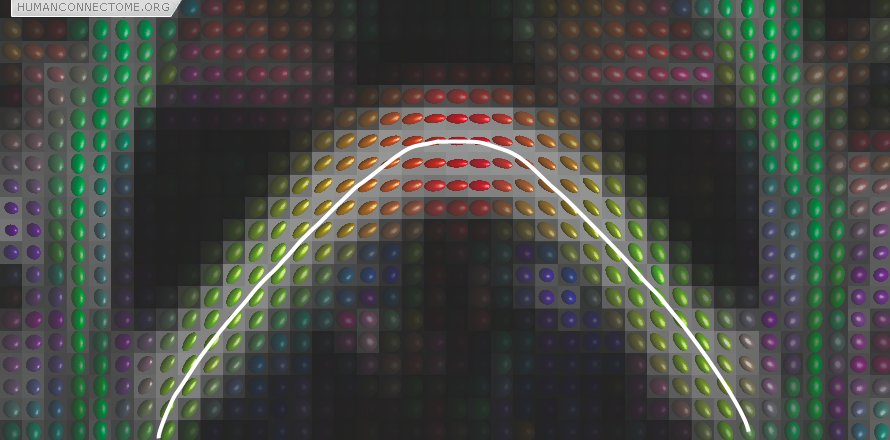
\includegraphics[width=4.5cm]{tensor_trajectory.jpg}
%  \caption{Tracking from tensor direction information}
%  \label{Fig:tracking}
%\end{figure}
%The last step is coregistration from native space to MNI (Montreal Neurological Institute)~\footnote{\url{http://www.mni.mcgill.ca/}} space. The reason is that all these tractographies were initially in native space or space of scanner. Because each measurement has it own coordinator, and this makes doctors or neuroscientists very difficult to compare, integrate or further study the tractography (see in figure ~\ref{Fig:sub1sub9coregister}). They are needed to be warped into the common space. In the other way, registration is the process of transforming from native space into the coordinate system~\cite{zvitia2010coregistration}. More detail about these steps can be found in ~\cite{bao2012dmri}.
%\begin{figure}
%  \centering
%  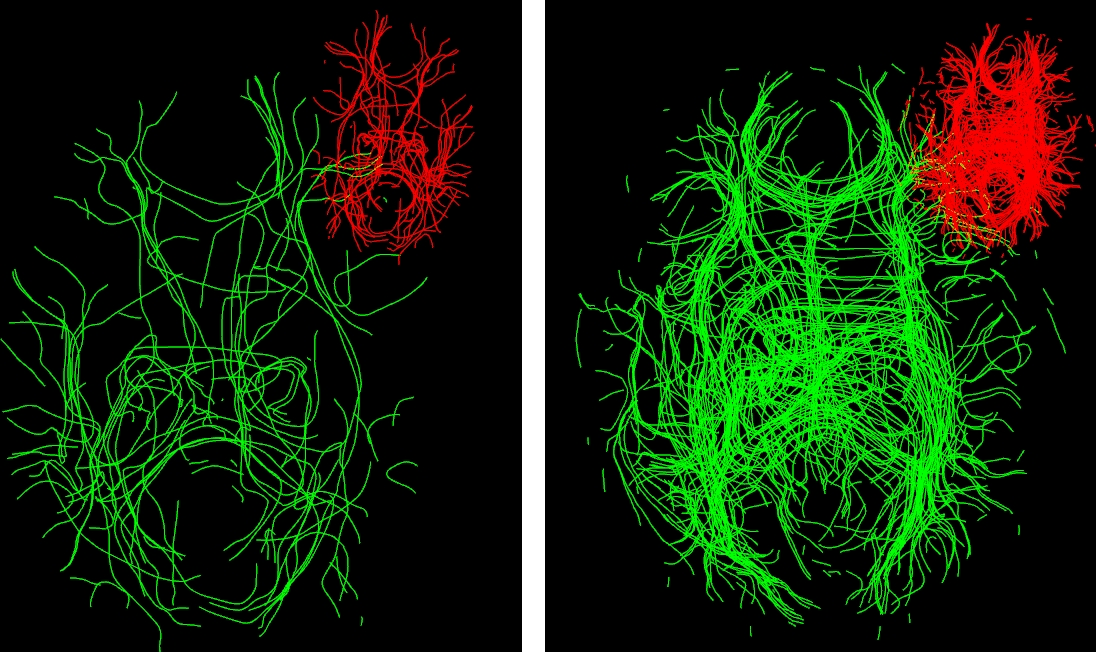
\includegraphics[width=4.5cm]{sub1_sub9_coregistering.jpg}
%  \caption{Tractography before(green) and after(red) the coregistration. Subject 1(left) and 9(right) of Cambrigde dataset}
%  \label{Fig:sub1sub9coregister}
%\end{figure}
\subsection{Tractography dissimilarity approximation}
\label{subsec:result_dissimilarity}
%Due to the lack of time, up to present, we only had experiment on dissimilarity approximation for tractography. 
In this section we describe the assessment of the degree of approximation of the dissimilarity representation across different prototype selection policies and different numbers of prototypes \cite{olivetti2012approximation}. The aim is to investigate the trade-off between accuracy and computational cost. The robustness of the method is checked first using simulated data, and then on the real tractography. But in the following, we only describe the experiment on real dMRI data. More detail about these experiments can be found in our recent publication~\cite{olivetti2012approximation} at PRNI-2012~\footnote{http://www.mlnl.cs.ucl.ac.uk/prni2012/} %The experiments are carried out on real tractographies reconstructed from dMRI recordings of the human brain.

We estimated the dissimilarity representation over real tractography data from dMRI recordings %of the MRI facility 
at the Cognition and Brain Sciences Unit, Cambridge, United Kingdom. The dataset consisted of $12$ healthy subjects; $101$ ($+1$, i.e. $b=0$) gradients; $b$-values from 0 to 4000; voxel size: $2.5 \times 2.5 \times 2.5 mm^3$. 
In order to get the tractography, 
% we computed the single tensor reconstruction (DTI) and created the streamlines using EuDX, 
we used the deterministic tracking algorithm~\cite{garyfallidis2012towards}.
% from the DiPy~\footnote{\url{http://www.dipy.org}}library. 
We obtained two tractographies using $10\times 10^3$ and $3\times10^6$ random seeds respectively. The first tractography consisted of approximately $10^3$ streamlines and the second one of $3\times 10^5$ streamlines. We used all three policies of choosing prototype: random, FFT and SFF. An example of a set of prototypes from $3\times10^5$ streamlines is shown in figure~\ref{fig:streamlines}. As the distance between streamlines we chose the most common one, i.e. the mean average minimum (MAM) distance from~\cite{zhang2008identifying} defined as $d_{mam}(s,s') = \frac{1}{2}(\delta(s,s') + \delta(s,s'))$ where
\begin{equation}
  \label{eq:mam_distance}
  \delta(s,s') = \frac{1}{|s|} \sum_{\mathbf{s}_{i} \in s}
    \min_{\mathbf{s'_j} \in s'} ||\mathbf{s}_i - \mathbf{s'}_j||_2.
\end{equation}
As shown in figure~\ref{fig:correlation_1K}(left), in the case of the $10^3$-streamline tractography, both FFT and SFF ($c = 3$) had significantly higher correlation than the random sampling for all numbers of prototypes considered. We confirmed that the SFF selection policy is an accurate approximation of the FFT policy for tractographies. Moreover we noted that after $15-20$ prototypes the correlation reached approximately $0.95$ on average ($60$ repetitions) and then slightly decreased indicating that a little number of prototypes was sufficient to reach a very accurate dissimilarity representation.
\begin{figure}
  \centering
  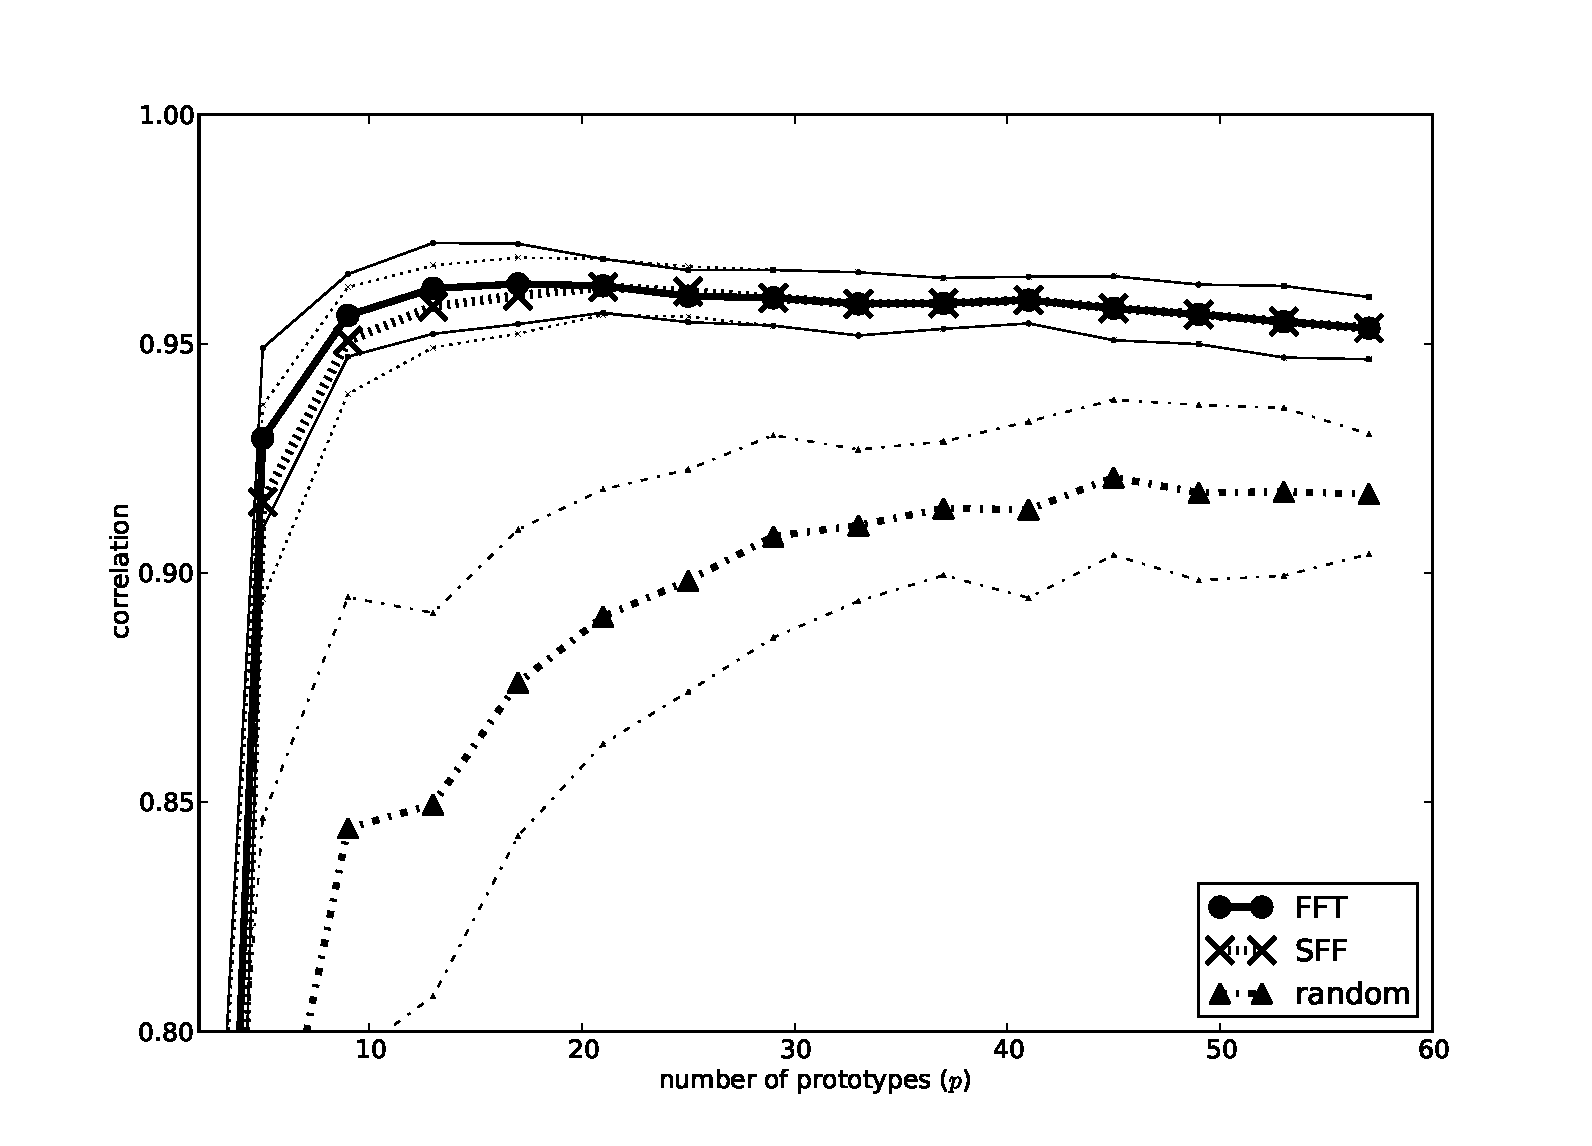
\includegraphics[width=4.5cm,height=3.85cm]{120323_file_120322_15h_subj1_60_4pro_c10_500tracks_allpairs_alltracksforpro_score_gen_9line_new.pdf}
  \includegraphics[width=4.1cm,height=3.85cm]%[bb=5 -5 80 80][bb=5 5 40 40]%
  {120323_file_120322_15h_subj1_100_5pro_c10_1000tracks_allpairs_alltracksforpro_score_gen_9lines.pdf}
  \caption{The correlation between of $d$ and $\Delta_{\Pi}^d$ over a
   tractography for different prototype selection policies: $\mathbf{10^3}$ streamlines (left) and $\mathbf{3\times 10^5}$ streamlines (right).}
  \label{fig:correlation_1K}
\end{figure}
%\begin{figure}
%  \centering
%  \includegraphics[width=6.5cm,height=3.85cm]%{120323_file_120322_15h_subj1_100_5pro_c10_1000tracks_allpairs_alltracksforpro_score_gen_9lines.pdf}
%  \caption{The correlation between of $d$ and $\Delta_{\Pi}^d$ for a
%    full tractography of $\mathbf{300K}$ streamlines for the random and SFF
%    prototype selection policies.}
%  \label{fig:correlation_300K}
%\end{figure}
Figure~\ref{fig:correlation_1K}(right) shows the correlation between SFF and the random policy when the tractography has $3\times 10^5$ streamlines, i.e. the standard size of a tractography from current dMRI recording techniques. In this case, FFT was impractical to be computed because it required approximately $15$ minutes on a standard desktop computer for a single repetition when $p=60$. The cost of computing SFF was instead the same of the case of $10^3$ streamlines, as its computational cost depended only on the number of prototypes. It took $\approx 2$ seconds on standard desktop computer when $p=60$ to compute one repetition. We observed that for $3\times 10^5$ streamlines, SFF significantly outperformed the random policy and reached the highest correlation of $0.96$ on average ($60$ repetitions) for $15-25$ prototypes. Note that the figures presented in this section refers to data from subject $1$ of the dMRI dataset. We conducted the same experiments on other subjects obtaining equivalent results. 

All of the results from both simulated data and real tractography data reached correlation $\geq 0.95$, showing a strong evident that dissimilarity approximation works well for preserving the relative distances. We advocate that the dissimilarity representation can produce compact feature spaces for the tractography. Moreover we strongly suggest the use of the SFF policy to obtain an efficient and effective selection of the prototypes.
\subsection{Spaghetti: an interaction visualization tool for tract segmentation}
\label{subsec:resul_spagheti}
In this part, we present a streamline interaction visualization tool, called Spaghetti, which is the implementation of the framework in figure~\ref{fig:ov_tool}. But until now, we have not integrated the hypo generation step in this tool yet. It is supposed to use the whole tractography $\mathbb{T}$ instead of a set of candidates $\mathcal{T}$.
%The main purpose of this scientific tool is to support medical practitioners to do the tract segmentation task more easy.
% Be honestly, interacting with tractography is a difficult procedure for various reasons: (a) tractographies are usually represented by hundreds of thousands of intertwined streamlines see~\ref{fig:tractography}; (b) data sets are often cluttered with noisy tracks, i.e. tracks which have no relevance in anatomy; (c) the size of the entire tractography is often too large to load in the memory of the graphics card; (d) navigating specific regions of a tractography in $3D$ space is cumbersome because of the unique shape characteristics of the streamlines. We build up an interactive tool that solves these problem.
%of interacting with tractographies by creating real-time simplifications in terms of the underlying bundle structures. 
The process that we propose works recursively: starting from a small number of clusters of streamlines the user decides which clusters to explore. Exploring a cluster means that the application re-clusters its content at a finer grained level or provides the content (means streamlines) of that cluster. In another words, the users change the level of abstraction and we provide cluster representatives of new clusters according to that level. % they want to look at the tractography, 

As the distance between streamlines, beside the MAM (equation~\ref{eq:mam_distance}, we also use the MDF (minimum average direct flip)
%$d_{mdf}(s,s') = min(\delta_{direct}(s,s'),\delta_{flipped}(s,s'))$
\begin{equation}
\label{eq:mdf_distance}
	d_{mdf}(s,s') = min(\delta_{direct}(s,s'),\delta_{flipped}(s,s'))
\end{equation}
with $\delta_{direct}(s,s') = \frac{1}{k} \sum_{i=1}^{k} 
	||\mathbf{x}_{i} - \mathbf{x'}_i||_2.$
and $\delta_{flipped}(s,s') = \frac{1}{k} \sum_{i=1}^{k} 
	||\mathbf{x}_{i} - \mathbf{x'}_{k-i}||_2.$
%\begin{equation}
%\label{eq:dirrect}
%	d_{direct}(s,s') = \frac{1}{k} \sum_{i=1}^{k} 
%	||\mathbf{x}_{i} - \mathbf{x'}_i||_2.
%\end{equation}
%\begin{equation}
%\label{eq:dirrect}
%	d_{flipped}(s,s') = \frac{1}{k} \sum_{i=1}^{k} 
%	||\mathbf{x}_{i} - \mathbf{x'}_{k-i}||_2.
%\end{equation}
where $k$ is the number of points $\mathbf{x}_{i}$ on the two tracks $s$ and $s'$.
%\begin{equation}
%\label{eq:mam}
%	MAM_{mean}(s,s') = \frac{1}{2}(d_{mean}(s,s') + d_{mean}(s',s))
%\end{equation}
%\begin{equation}
%\label{eq:mean}
%	d_{mean}(s,s') = \frac{1}{k} \sum_{i=1}^{k}	d(\mathbf{x}_{i},s')
%\end{equation}
%\begin{equation}
%\label{eq:min}
%	d(\mathbf{x},s) = min_{j=1,\ldots,k}||\mathbf{x} - \mathbf{x'}_{j}||_2
%\end{equation}
In this software, currently we use the fast clustering algorithm proposed in~\cite{garyfallidis2012quickbundles}, called QuickBundle(QB). The reason is that QB is very simple, easy to implement and very fast. However, every time user change the level of abstraction, we need to re-run QB to get the new clusters. It is one of the drawbacks of the current version of Spaghetti.

The application starts visualizing the brain as a set of a few cluster representative.
%, i.e. the cluster representatives.
Each representative track acts as the access point to the streamlines within that cluster and allows the user to address this portion of the tractography as a single unit, which we call "bundle of interest" (BOI). After visually inspecting the simplified tractography the user interactively selects one or more representative tracks and explores them.
%When one or more representative tracks are selected the user can see the content of the related clusters. 
In order to explore the detailed %structure of content 
of the selection, the user may ask to re-cluster the selected BOIs, and possibly further refine the initial selection.
% into smaller clusters in order to address and possibly further refine the initial selection. 
%This procedure can repeat until user satisfies with the the local structures result.
After selecting one or more of the small clusters through their representatives the user can repeat the visual inspection step, and the re-clustering step as required in order to unveil the local structures.
\begin{figure}
	\centering
	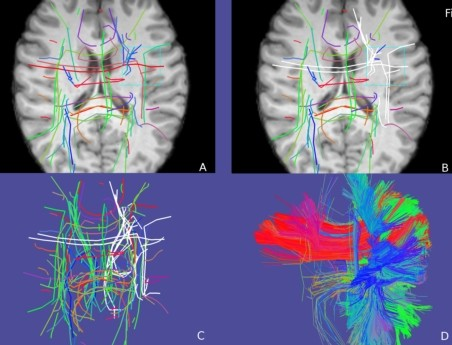
\includegraphics[height=3.85cm]{spaghetti1.jpg} %width=7.5cm
	\caption{Streamline interaction with Spaghetti: the initial representatives (A); some selected clusters in white color (B); only representatives without slices (C); exploring representatives by hundred of streamlines (D)}
  \label{fig:spaghetti}
\end{figure}
Beside the capability of interacting with streamlines, in this tool we also provide function of visualizing slices of structural volumes (see figure~\ref{fig:spaghetti}). The volume is aligned in the same space (e.g standard space) of the tractography.
% We also provide functions to move/hide these slicers . 
This enables medical practitioners and researchers to meaningfully navigate the entire space of the tractography related to anatomy. The detail of this tool can be found in our publication~\cite{garyfallidis2012software}  at OHBM-2012\footnote{Organization for Human Brain Mapping 2012~\url{http://www.humanbrainmapping.org/OHBM2012/}}
 %These representative tracks are provided by a very fast tractography clustering algorithm. %called QuickBundles~\cite{garyfallidis2012towards} which can cluster thousands of tracks in milliseconds. 
%~\cite{garyfallidis2012quickbundles}
%\subsection{Clinical diagnosis applications}
%Some text here
%\textbf{Diagnosis ALS disease}
%Some text here
%\textbf{Other disease here}
%Some text here
\subsection{Clinical diagnosis application: the difference of Corticol Spinal Tracts between a healthy and an ALS-diseased brain}
\label{subsec:result_ALS}
In this part, we try to demonstrate the usefulness of tract segmentation in clinical study. 
%Traditionally, diagnostic decision making has involved using evidence provided by patient's data coupled with physician's priori experience. Up to now, it is still very much an art for many physicians due to a lack of quantitative tools and measurements. 
The aims of this work are to: first, finding the differences of the Corticol Spinal Tracts (CST) between a healthy brain and an ALS (Amyotrophic Lateral Sclerosis) diseased brain based on tract quantification; and second present a general framework for clinical diagnosing based on the differences between two folders of interesting tracks.
%1) describe a process to perform tractography from discrete measured diffusion tensor MRI data of ALS-2012 dataset; 
%1) present a general framework for finding the differences between two folders of tracks based on tract quantification; and 2) demonstrate this process in finding the differences of the Corticol Spinal Tracts (CST) between a healthy brain and a patient.
%\begin{figure}
%  \centering
 % 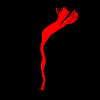
\includegraphics[bb=0 0 140 150]{201CTS1Mleft_1.png}
 % 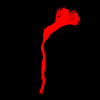
\includegraphics[bb=0 0 140 150]{201CTS3Mleft_1.png}%[bb=0 0 200 300]
 % \caption{The left CTS segmentation of control 201 in the dataset ALS\underline{ }Nivedita. The left image is the segmentation from the 1M tractography and has $154$ tracts. While the right is one from 3M tractography and the number of tracts is $487$.}
 % \label{fig:CTS_201_left}
%\end{figure}
\begin{figure}
  \centering
  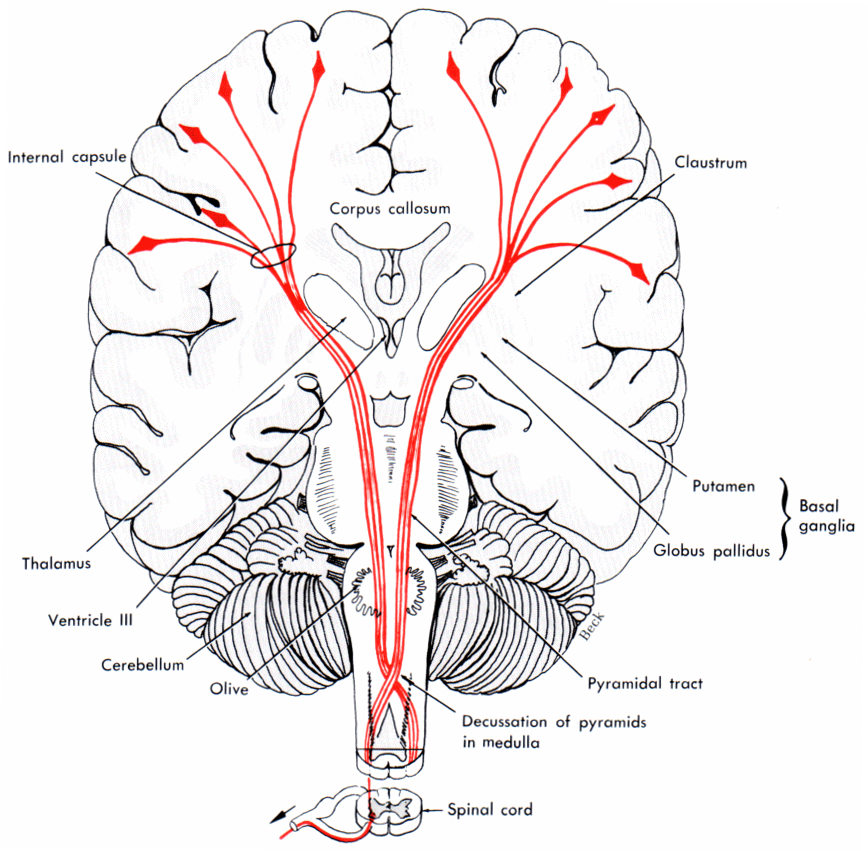
\includegraphics[width=4.2cm,height = 3.85cm]{CST.png}
  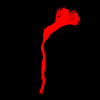
\includegraphics[bb=5 -5 80 80]{201CTS3Mleft_1.png}
  \caption{Left - the Cortico Spinal Tracts in general. Right - the left CST segmentation of the control 201 in the dataset ALS}%\underline{}Nivedita}%, from 3M tractography and the number of tracts is $487$}
  \label{fig:CST}
\end{figure}
%ALS, also known as motor neurone disease or Lou Gehrigs disease, is a fatal, progressive neuromuscular disease that attacks the motor neurons controlling voluntary movement. The result is wasting and atrophy of muscles, leading to difficulties in speaking or swallowing, stumbling, permanent fatigue and cramping, amongst other symptoms. 
\\\textbf{\textit{ALS}}, also known as motor neurone disease or Lou Gehrigs disease, is a progressive neurodegenerative disease that affects nerve cells in the brain and in the spinal cord. 
%Motor neurons reach from the brain to the spinal cord and from the spinal cord to the muscles throughout the body. 
As motor neurons degenerate, they can no longer send impulses to the muscle fibers that normally result in muscle movement. The result is wasting and atrophy of muscles, leading to difficulties in speaking, swallowing, stumbling, etc. %permanent fatigue and cramping, amongst other symptoms. Due to that fact that 
Because ALS disease involves to the nerve cells in \textit{\textbf{CST}}, in this part, we only focus on this CST tract.
%for diagnosing ALS we need to know the difference of CST between a healthy and an ALS-diseased brain. 
Usually, CST starts from the cerebral cortex, and terminates in the spinal cord. Note that fibers after crossing over from one side to the other
%, in the medulla, 
continue downward in the lateral corticospinal tract on the opposite side and go to muscles (see figure~\ref{fig:CST}-left). %Each crossed corticospinal tract, therefore, conducts motor impulses from one side of the brain on interneurons or anterior horn motoneurons on the opposite site of the cord. 
That is the reason why impulses from one side of the cerebrum cause movements of the opposite side of the body.

CST segmentation was done by doctors using Spaghetti tool on the ALS dataset, recorded with a $3T$ scanner at Utah Brain Institute. This dataset consisted of $12$ healthy controls and $12$ subjects; $64$ ($+1$, i.e. $b=0$) gradients; $b$-values $1000$; voxel size: $1. \times 1. \times 1. mm^3$. For creating tractography, we used the same algorithm in section~\ref{subsec:result_dissimilarity}, with $3\times 10^5$ random seeds. An example of CST segmentation from ALS dataset is in figure~\ref{fig:CST} (left). As the result, we had $48$ segmentations ($24$ of patients including $12$ left CST and $12$ right CST; and similar for controls).

From the prior knowledge of neuroscientists and doctors, there is an evidence about the reducing of the number of fibers in CST of ALS patients compared with control people. It is also the same situation with the volume of CST. Beside,
% the number of fibers and the volume, 
fractional anisotropy (FA) and mean diffusion (MD) also play an important role for recognizing the ALS disease. Following are some quantitative features which may effectively affect on ALS patients: \textit{fiber count} - the number of streamlines belonging to CST; \textit{fiber length} in $mm$ (min, max, mean length); \textit{fiber volume} - number of voxels occupied by all streamlines or the bounding geometry cylinder of CST; \textit{fiber density} - ratio between fiber count and voxel number; \textit{fragmentation} - %can be quantified by the 
ratio between fiber count and the volume; \textit{fractional anisotropy (FA)} - defined as mean value of the standard deviation in the three eigenvalues and in the range $0$ to $1$
	\begin{equation}
   FA=\frac{1}{\sqrt{2}}\frac{\sqrt{(\lambda_{1}-\lambda_{2})^{2}+(\lambda_{2}-\lambda_{3})^{2}+(\lambda_{3}-\lambda_{1})^{2}}}{\sqrt{\lambda_{1}^{2}+\lambda_{2}^{2}+\lambda_{3}^{2}}}
   \label{eq:FA}	
\end{equation} 
and \textit{mean diffusion (MD)} - the average diffusion rate in all directions% $MD=\frac{1}{3}(\lambda_{1}+\lambda_{2}+\lambda_{3})$ 
	\begin{equation}
   MD=\frac{trace(DT)}{3}=\frac{\lambda_{1}+\lambda_{2}+\lambda_{3}}{3}
%	   MD=\frac{\lambda_{1}+\lambda_{2}+\lambda_{3}}{3}
   \label{eq:MD}	
\end{equation}
%
%\begin{itemize}
%	\item fiber count: the number of streamlines belonging to CST
%	\item fiber min/max/mean length: length in $mm$% for all streamlines belonging to CST
%	\item fiber volume: number of voxels occupied by all streamlines or the bounding geometry cylinder of CST
%	\item fiber density: ratio between fiber count and voxel number
%	\item FA: defined as mean value of the standard deviation in the three eigenvalues and in the range $0$ to $1$
%	\begin{equation}
 %  FA=\frac{1}{\sqrt{2}}\frac{\sqrt{(\lambda_{1}-\lambda_{2})^{2}+(\lambda_{2}-\lambda_{3})^{2}+(\lambda_{3}-\lambda_{1})^{2}}}{\sqrt{\lambda_{1}^{2}+\lambda_{2}^{2}+\lambda_{3}^{2}}}
%   \label{Equ:FA}	
%\end{equation}
%	\item MD: the average diffusion rate in all directions 
%	\begin{equation}
%   MD=\frac{trace(DT)}{3}=\frac{\lambda_{1}+\lambda_{2}+\lambda_{3}}{3}
%	   MD=\frac{\lambda_{1}+\lambda_{2}+\lambda_{3}}{3}
%   \label{Equ:MD}	
%\end{equation}
%	\item fragmentation: %can be quantified by the 
%	ratio between fiber count and the volume
%\end{itemize}
where ($\lambda_{1}, \lambda_{2}, \lambda_{3}$) is eigenvalues of diffusion at a given voxel.
\\After calculating the value of these features, we did a $t-test$ on each set of left and right. It showed that, in the right CST, fiber number significantly decreased $(p = 0.00042)$ in ALS patients ($mean_{fiber-number} = 294$) compared with controls ($mean_{fiber-number} = 640$). In contrast, patients had the fiber min length slightly higher then controls ($p=0.07$, patients: $mean_{min-length}= 74.25$ and controls: {$mean_{min-length} = 53.9$). Moreover, the volumn of the left CST dramatically diminished ($p=0.0034$) between patients ($mean_{volumn}=6038$) and healthy peoples ($mean_{volumn}=4230$). These are just some preliminary results and it needs more investigation to confirm the difference between healthy and ALS-diseased brain. But it also shows an strong evidence that the tract segmenation has a bright capability for applying in clinical diagnose application.
%The CST converges in the subcortical white matter (corona radiata) and courses through the posterior limb of the internal capsule, the cerebral peduncle of the midbrain, the ventral pons (basis pontis), the ventral surface of the medulla, decussate in the lower medulla (pyramidal decussation). The figure~\ref{fig:CST} shows a visualization of CST. In this figure, axons that compose pyramidal tracts come from neuron cell bodies in the cerebral cortex. After they descend through the internal capsule of the cerebrum and the white matter of the brainstem, about three fourths of the fibers decussate cross over from one side to the other, in the medulla. After that, the fibers continue downward in the lateral corticospinal tract on the opposite side of the cord. Each crossed corticospinal tract, therefore, conducts motor impulses from one side of the brain on interneurons or anterior horn motoneurons on the opposite site of the cord. That is the reason why impulses from one side of the cerebrum cause movements of the opposite side of the body.

%\vspace{-2mm}
\section{Conclusion}
\label{sec:conclusion}
\vspace{-2mm}
%the contribution of the paper
In this paper, we presented a method for addressing the problem faced when attemping to interactively visualize a large dataset. The core principle behinds the framework was to choose \emph{multiple scales for representing} the data from the hierarchical clustering. Moreover, we also proposed a function to evaluate the goodness of each chosen scale based on the concept of \emph{split factor}. We instantiate this framework with an application of building the interactive visualization large dMRI data in the procedure of tractogaphy segmentation, and provide concrete result on it performance. Experiments have shown that our method provide a significant improvement for visualization the large data at different scales, which verifies the effectiveness of the interactive hierarchical visualization. Beside, we are convinced that this method can be easily integrated to any current display techniques without having to vary the data or the interactive exploration tool. 

%what is the limitation of our proposed methods and/or future works
\vspace{1mm}
As mention is the section~\ref{sec:methods}, the level of detail of each cluster, $s(C_i)$, can be computed based on radius or heigh~\cite{yang2003interactive}. In this paper we choose the multiple scales only based on the heigh of cluster. The same job but based on the radius needs to be investigated. Moreover, this work is a part of an going resarch project focusing on computer-aided tractography segmentation, where machine learning techniques are used to assist medical practitioners to do the segmentaion task more easily, flexibly  and effectively. In the future, we want to further improve the interactive segmentation tool by providing the function of adding or eleminating data points $x$ into or from the current dataset $\mathcal{X}$, and updating the visualization result without re-run the clustering algorithm.

\vspace{-3mm}


The structure of this paper is as follows. In Section~\ref{sec:state_of_the_art}, we introduce the basic background of dMRI and tractography segmentation. The latter part of this section briefly summarizes some current trends in segmentation tractography task. Section ~\ref{sec:problem_statement} formally presents the problem of clustering a tractography, which is one of the contribution of this project. In Section~\ref{sec:solution}, we describe the proposed solution for online clustering tractogprahies. In this part, we also illustrate the dissimilarity representation based on the most common streamline-streamline distance functions. In Section~\ref{sec:preliminary_results}, we present the preliminary result of our experiment about the dissimilarity approximation on a real dMRI dataset from the University of Cambridge (UK). An interactive visualization software tool for segmentation, called \textbf{Spaghetti}, is also presented. Moreover, one clinical application to support the diagnosing of the ALS-disease is also introduced. %(this work has not finished yet, and will be presented detail in near future). 
The last section, Section ~\ref{sec:conclusion}, discusses results
% supporting the claim that machine learning techniques are straightforward and effective for the tract segmentation task. In this part, we also 
and points out some future works.% oriented on clinical applications.
%for applying the tractography segmentation complementing the segmentation task.
